\graphicspath{{Chapters/PCS/Figures/}}

\chapter{Photon Correlation Spectroscopy in a Diamond Anvil Cell} \label{chap:PCS}
\section{Justification}\label{sec:PCSIntro}

\sect \ref{sec:probes} describes several probes commonly implemented to measure molecular dynamics in glass-forming systems as the timescale associated with structural relaxation changes by as much as fifteen orders of magnitude while the liquid vitrifies into a glass. Wolynes and Lubchenko assert in their discussion of Dielectric Spectroscopy (DS) that this technique is uniquely suited to track molecular dynamics in glass-forming systems over this large dynamic range. Indeed, when taken as a whole, the multitude of methods that fall under the banner of DS provide an astonishing range of measurement for relaxation times from $\tau \approx 1 \,\si{\nano\second}$ up to $\tau > 1000 \,\si{\second}$\nolinebreak\cite{Wolynes}. However, many of these methods do not lend themselves well to the geometric constraints and experimental limitations of a diamond anvil cell (DAC) or other high-pressure apparati. For example, reflection or transmission techniques require that the sample be arranged in a macroscopic coaxial configuration. The methods that may lend themselves well—most notably frequency response and time-domain analysis—are only now being developed in the context of the DAC\cite{Peng,Chan,Ransom2017DACDielectric}.

As shown in \fig \ref{figure:Probes}, depolarized photon correlation spectroscopy (DPCS) covers a dynamic range similar to that of conventional dielectric spectroscopy (DS) frequency-response analysis, extending in principle from approximately $10 \,\si{\nano\second}$ to beyond one thousand seconds, and provides a direct probe of the structural $\alpha$-relaxation. When combined with depolarized Brillouin light scattering (DBLS), the accessible dynamic range of light scattering techniques is extended by several additional decades toward shorter times, approaching a total span of nearly 15 orders of magnitude. A relatively narrow gap remains between the fastest dynamics accessible to DPCS and the slowest dynamics probed by DBLS. In principle, this intermediate regime is accessible via dielectric spectroscopy in the radio-frequency (RF) range; however, such high-frequency dielectric measurements have proven difficult to implement under the constraints of high-pressure diamond anvil cell environments and have seen limited application in this context.  

Although both DPCS and DS offer comparable windows for measuring molecular dynamics, they differ fundamentally in how those dynamics are accessed. DPCS is a passive technique that probes spontaneous fluctuations arising from the stochastic thermal evolution of the system, whereas dielectric spectroscopy is inherently a driven measurement, relying on an externally applied electric field to induce dipolar reorientation. While linear-response conditions are typically assumed, the driven nature of DS raises the possibility that the modes most strongly excited by the applied field may not uniquely correspond to the collective structural relaxation of the material.

Additionally, DPCS does not require electrode structures within the sample volume; only optical access is needed, making it a particularly accessible option for extending measurements of structural relaxation into the diamond anvil cell. Despite these differences, both methods are worthy of development, as they possess complementary strengths and limitations.

Dielectric spectroscopy provides a direct probe of structural relaxation only when the dielectric susceptibility faithfully reflects the orientational dynamics of the liquid under study. In such cases, the primary dielectric loss peak may be identified with the bulk $\alpha$-relaxation. However, this correspondence is not guaranteed. DS is intrinsically sensitive to dipolar reorientation, and when molecular dipoles are associated with specific subunits or segments, the measured response may be dominated by local or segmental dynamics rather than collective structural rearrangement. 

This limitation is well illustrated in polymeric systems, where dipole moments may be associated with specific molecular subunits rather than the global structure. In such cases, dielectric spectroscopy can be dominated by local or segmental dynamics that are decoupled from collective structural relaxation. For example, in poly(dimethylsiloxane) (PDMS), the dipole moment is oriented transverse to the polymer backbone, such that the dielectric response reflects only segmental motion rather than global chain dynamics\cite{Wrzesinska2020}. While polymeric systems provide a particularly clear manifestation of this effect, the underlying issue is more general: whenever dipolar reorientation does not uniquely track collective structural rearrangement, the dielectric $\alpha$-process may not faithfully represent bulk relaxation. This motivates the use of complementary probes that couple more directly to density or orientational fluctuations of the material as a whole.

Depolarized photon-correlation spectroscopy couples to fluctuations in the anisotropic component of the molecular polarizability tensor. As a result, DPCS is inherently sensitive to orientational and structural dynamics associated with collective molecular rearrangement, while remaining insensitive to purely isotropic density fluctuations. This selectivity provides a complementary view of structural relaxation dynamics, though it too comes with inherent limitations, perhaps the most significant being that the molecular system must exhibit a sufficiently strong polarizability anisotropy to generate a measurable depolarized scattering signal.

Molecules with extremely high symmetry, such as carbon tetrachloride or sulfur hexafluoride, lack significant anisotropic (off-diagonal) components of the dielectric susceptibility tensor and therefore do not generate an observable depolarized scattering signal. While such highly symmetric systems rarely form molecular glasses due to their strong tendency toward crystallization, they provide a useful conceptual limit that illustrates the symmetry-imposed constraints of DPCS. 

Experimentally relevant glass formers typically exhibit some degree of molecular anisotropy.  The same geometric features that give rise to orientational frustration and enable glassy dynamics in the first place also tend to generate off-axis components of the dielectric susceptibility tensor. Consequently, glass-forming systems generally lend themselves to producing at least some measurable depolarized scattering signal.

Despite the respective limitations of both depolarized photon--correlation spectroscopy (DPCS) and dielectric spectroscopy (DS), many systems may lend themselves equally well to either probe, at least in principle. A clear illustration of this complementarity is provided by \textit{n}-propanol, which possesses a substantial dipole moment of 1.57~Debye~\cite[p.~9-48]{CRC1997} and is therefore well suited to dielectric measurements, while also exhibiting sufficient molecular anisotropy to produce a measurable depolarized scattering signal, as is commonly observed in comparable small-molecule glass-forming liquids~\cite[p.~114]{Berne}\cite{Brodin}. Although its polarizability anisotropy is smaller than that of aromatic liquids such as cumene, \textit{n}-propanol represents an intermediate case in which both dielectric spectroscopy and DPCS can probe relaxation dynamics in the liquid.

Notably, \textit{n}-propanol is a small, comparatively rigid molecule, and therefore does not exhibit the segmental or sub--chain dynamics that can complicate the interpretation of dielectric spectra in polymeric or highly flexible systems. Nevertheless, this does not guarantee that dielectric spectroscopy directly probes the structural $\alpha$--relaxation. In monohydroxy alcohols such as \textit{n}-propanol, the dielectric response is characterized by a nearly Debye-like relaxation, while mechanical and structural probes reveal markedly different relaxation behavior, indicating pronounced decoupling in both timescale and spectral shape. This decoupling has been attributed to the presence of hydrogen-bonded microheterogeneities within the liquid structure \cite{Angell2000}.

While this dielectric relaxation arises from intermolecular dipolar correlations, it does not directly correspond to the structural $\alpha$--relaxation. Consequently, DS in \textit{n}-propanol reflects collective dipolar fluctuations associated with hydrogen--bonded correlations, rather than providing a direct measure of bulk structural dynamics, and its amplitude and spectral shape may be influenced by the evolving network structure \cite{Davidson,Angell2000}.

\begin{figure}[!htbp]
	\centering
	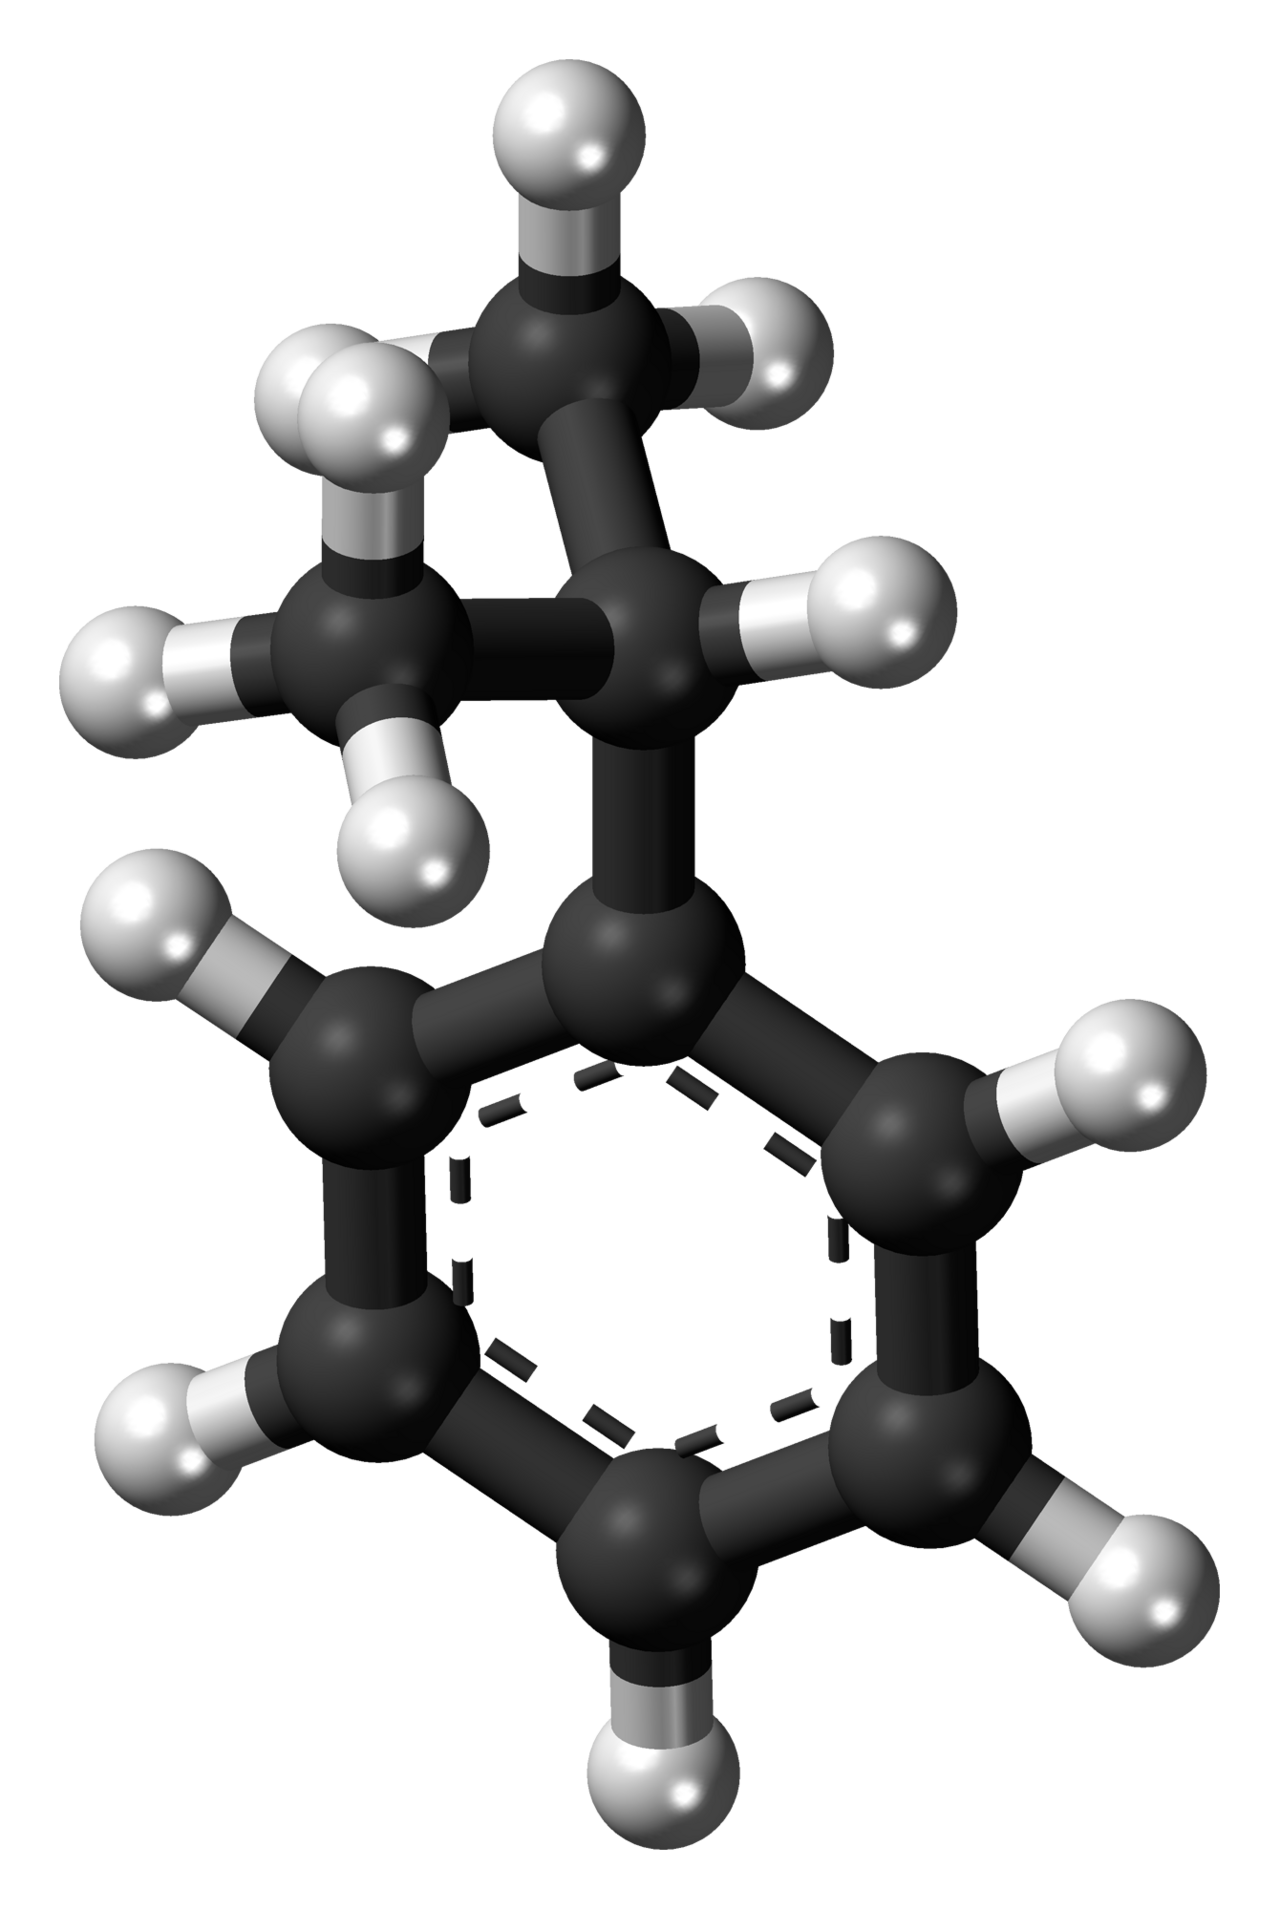
\includegraphics[width=0.35\textwidth]{Chapters/PCS/Figures/Cumene_3D_ball.png}
	\caption{Molecular structure of cumene (isopropylbenzene). The rigid aromatic ring contributes to a large polarizability anisotropy, while the absence of hydrogen bonding results in comparatively simple van der Waals–dominated relaxation dynamics.}
	\label{figure:CumeneStructure}
\end{figure}

Cumene (isopropylbenzene), shown in \fig\ref{figure:CumeneStructure}, represents a complementary case that is particularly favorable for both probes. Its rigid aromatic structure gives rise to a large polarizability anisotropy, making it exceptionally well suited to DPCS measurements, while the absence of hydrogen bonding or internal molecular flexibility ensures that its dielectric response, though weaker due to the modest permanent dipole moment, remains closely tied to the collective structural $\alpha$--relaxation. Consequently, although \textit{n}-propanol yields a weaker depolarized scattering signal and cumene a weaker dielectric response, both systems lend themselves naturally to investigation by either technique, with each probe accessing the same underlying structural relaxation dynamics. Even in such systems, DPCS may be a preferable probe simply because it requires only optical access to the sample.

In conclusion, in systems with strong molecular anisotropy but complex or heterogeneous dipolar dynamics, such as polymeric liquids or molecular systems with independently mobile dipolar subunits, dielectric spectroscopy may preferentially probe local or segmental relaxations rather than collective structural rearrangement. In these cases, DPCS remains directly sensitive to the bulk $\alpha$-relaxation, providing a direct probe of structural relaxation dynamics by accessing the stochastic thermal evolution of the system without coupling to driven, local modes \cite{Roland,Patterson}.

\begin{table}[!htbp]
	\centering
	
	\tabletitle{Representative molecular systems illustrating DS and DPCS sensitivity}
	\vspace{0.5em}
	
	\begin{tabular}{lccccc}
		\hline
		Molecule & Glass Former & $\chi_{i\neq j}$ & DS Sensitivity & Anisotropic Signal \\
		\hline
		Cumene (isopropylbenzene) & Yes & Large & Direct $\alpha$ & Very strong \\
		\textit{n}-Propanol & Yes & Moderate & Decoupled & Moderate \\
		Poly(vinyl acetate) & Yes & Large & Segmental & Strong \\
		Glycerol & Yes & Moderate & Mixed & Moderate \\
		\hline
		Carbon tetrachloride (CCl$_4$) & No & Vanishing & Weak & Weak \\
		Sulfur hexafluoride (SF$_6$) & No & Vanishing & Weak & Weak \\
		\hline
	\end{tabular}
	
	\label{tab:DSvsDPCS}
	
	\tabledescription{Off-diagonal $\chi_{i\neq j}$ denotes the relative magnitude of anisotropic contributions to the dielectric susceptibility tensor responsible for depolarized scattering. Highly symmetric molecules are included as conceptual reference cases, though their poor glass-forming ability limits their relevance here. In such systems, DPCS yields little to no measurable depolarized signal due to the near-isotropy of the susceptibility tensor, and DS shows no meaningful correlation with collective structural relaxation. For \textit{n}-propanol, ``Decoupled'' indicates that the dominant dielectric relaxation does not correspond directly to the structural $\alpha$--process, but instead reflects dipolar dynamics associated with hydrogen--bonded correlations.}
\end{table}

Having established the complementary strengths and limitations of dielectric spectroscopy and depolarized photon-correlation spectroscopy, it is important to emphasize the experimental challenges associated with extending DPCS into the diamond anvil cell. The most significant of these is the exceedingly small sample volume, typically on the order of $\sim 10\,\si{\nano\liter}$. In conventional cuvette-based light-scattering experiments, the scattered signal is collected from an extended region illuminated by a focused beam that may span several hundred microns, resulting in effective scattering volumes on the order of a few nanoliters. In the DAC geometry, by contrast, the illuminated region is typically confined to only a few tens of microns.

Under these conditions, it is necessary to ensure that a sufficient number of statistically independent scatterers contribute within the effective scattering volume so that the detected field obeys the Gaussian statistics assumed by photon correlation spectroscopy. This consideration is particularly relevant in experiments where scattering arises from a low number density of discrete mesoscopic scatterers, such as microspheres undergoing Brownian motion in a host liquid, for which the effective number of scatterers within the probe volume may be limited. For homogeneous liquids, however, light scattering originates from ubiquitous thermal density fluctuations, and even picoliter-scale scattering volumes contain an effectively macroscopic number of dynamically independent fluctuators. As a result, the Gaussian-field assumption remains well satisfied for pure liquids, provided that parasitic scattering from the gasket or diamond anvils is adequately suppressed.

This brings us to another concern regarding DPCS in a DAC\textemdash stray spectral reflections from every optical interface, together with unavoidable scattering from the gasket material, are collected alongside the desired signal. As a result, isolating the true scattering volume and suppressing background contributions is a dominant experimental challenge.

Herbst \etal addressed many of these difficulties in their effort to extend photon correlation spectroscopy (PCS), identical in application to DPCS but without polarization analysis, into the DAC as a probe of viscosity at high pressures \nolinebreak\cite{Herbst}. By analyzing the Brownian motion of polystyrene spheres suspended in the liquid, they obtained reasonable agreement with known values of methanol viscosity at pressures up to 2.9~GPa. Although successful, this approach has not reappeared in the literature since its publication, likely because the experimental complexity is disproportionate to its limited applicability: the method probes viscosities only up to approximately 90~cP.

In principle, the accessible viscosity range could be extended by employing smaller tracer particles and performing longer-timescale autocorrelations. Nevertheless, this approach remains orders of magnitude removed from the glass-transition regime, where viscosities reach $10^{15}$~cP. Indeed, in the same year, Cook, working with Herbst \etal, demonstrated centrifuge rolling-ball viscometry in a DAC at viscosities exceeding $10^{9}$~cP \nolinebreak\cite{Cook}. However, rolling-ball techniques are inherently limited to viscosities for which a macroscopic object can traverse the liquid within a practical experimental timescale and therefore cannot be extended to the glass transition.

By contrast, DPCS in a DAC could, at least in principle, access the glass transition and beyond if correlation spectra could be obtained directly from intrinsic density fluctuations of the pure liquid, rather than from nanoparticles suspended within it. The fundamental obstacle to this approach is the extremely weak scattering intensity associated with such fluctuations. In the Rayleigh regime, the intensity of light scattered from spherical particles scales with the sixth power of the particle radius \nolinebreak\cite{Sinclair}. Consequently, the scattering intensity arising from intrinsic density fluctuations, whose characteristic correlation lengths remain nanometric even in the presence of cooperative dynamics, will be many orders of magnitude weaker than that obtained from the 90~nm polystyrene spheres used by Herbst \etal. All of the challenges associated with small sample volumes are therefore dramatically amplified when attempting to extend PCS or DPCS measurements to pure liquids in the DAC.

One goal of this chapter is to describe the process of extending depolarized photon-correlation spectroscopy (DPCS) into the diamond anvil cell, thereby establishing a new probe of slow dynamics at very high pressures, up to and beyond the glass transition. Given the severe experimental constraints outlined above, it is essential to begin with a molecular system that maximizes the depolarized scattering signal. Aromatic liquids such as isopropylbenzene (cumene), with their large anisotropic polarizability arising from the benzene ring, produce exceptionally strong depolarized scattering signals and therefore represent near-optimal candidates for such a proof-of-concept study.

Cumene, a simple van der Waals–bonded glass-forming liquid, was selected both for this reason and for the availability of independent fast-dynamics data from Brillouin light-scattering measurements \cite{Li1995CumenePRL}. Together, these data allow characterization of relaxation dynamics over an exceptionally broad range of timescales, spanning from tens of picoseconds to hundreds of seconds. In addition, a separate study provided direct measurements of the pressure dependence of the glass-transition temperature via the \tgp method \cite{RansomPRL} described in \chap \ref{sec:IGPintro}. Agreement among these independent probes provides strong evidence for the efficacy of DPCS as a reliable probe of slow dynamics at high pressures in a DAC.

As previously mentioned, the light scattered from intrinsic density fluctuations within a pure liquid was expected to be exceedingly weak compared to undesired sources such as specular reflections from the diamond surfaces and gasket interfaces. An initial attempt therefore assumed heterodyne operation, deliberately collecting both the desired scattered signal and accompanying elastic and surface-scattered light, with the latter serving as a local oscillator. The combined light was directed onto the photomultiplier tube (PMT), with neutral-density filters used to attenuate the total intensity to a safe count rate. A polarizer was employed primarily to isolate the depolarized component of the scattering signal required for DPCS; however, the finite extinction ratio of the cube polarizer used in this setup allowed a significant fraction of elastically scattered and specularly reflected light to pass through. In practice, the collected light comprised contributions from these sources, rendering a homodyne/heterodyne determination difficult. Under these conditions, it is perhaps not surprising that no correlation decay could be resolved even after several hours of data acquisition.

It was therefore clear that spatial filtering was required to reject as much of the residual local oscillator as possible. This, however, introduced a new problem\textemdash physically locating the scattering volume within an exceedingly large region of optical splash. A telescopic viewfinder could be lowered into place to image the interior of the DAC for alignment purposes, but this proved insufficient. The experimenter was still left to blindly raster the collected light across the pinhole in an attempt to isolate a correlation decay signal. Given the uncertainty regarding how long signal averaging would be required before a clear decay emerged, and the tedious nature of blindly rastering over a relatively large area, this approach was impractical.

The present effort to implement DPCS within a DAC can be viewed as an extension of the strategy first demonstrated by Demoulin \etal, who showed that time-domain correlation of scattered intensity provides direct access to structural relaxation on timescales spanning microseconds to seconds\nolinebreak\cite{Demoulin}. Their analysis of undercooled glycerol established the utility of the Cole--Davidson distribution in describing broad, nonexponential relaxation spectra. Later, Lindsey and Patterson demonstrated the correspondence between the Cole--Davidson and Williams--Watts functions, providing a practical means of translating between frequency- and time-domain analyses\nolinebreak\cite{Lindsey}. Taken together, these works justify the approach pursued here: by developing the experimental capability to isolate weak depolarized scattering from liquids under extreme confinement in a DAC, one gains a direct probe of structural relaxation that is theoretically continuous with both ultrasonic/frequency-domain results and with the broad body of photon correlation data analyzed in the time domain. Furthermore, high-pressure DPCS data provides direct access to structural relaxation dynamics in glass-forming systems that are closely related to those probed by DBLS in the frequency domain, which accesses much shorter time scales down to about a ps \cite{47,119}, with a narrow intermediate regime separating the two techniques.
\graphicspath{{Chapters/PCS/Figures/}}

\section{Experimental Details}\label{sec:PCSExp}

The complete experimental layout is shown in \fig \ref{figure:PCSsetup} and is described below along with the process of obtaining an autocorrelation signal.
\begin{figure}[!htbp]
	\centering
	\begin{tikzpicture}
		\node (img) {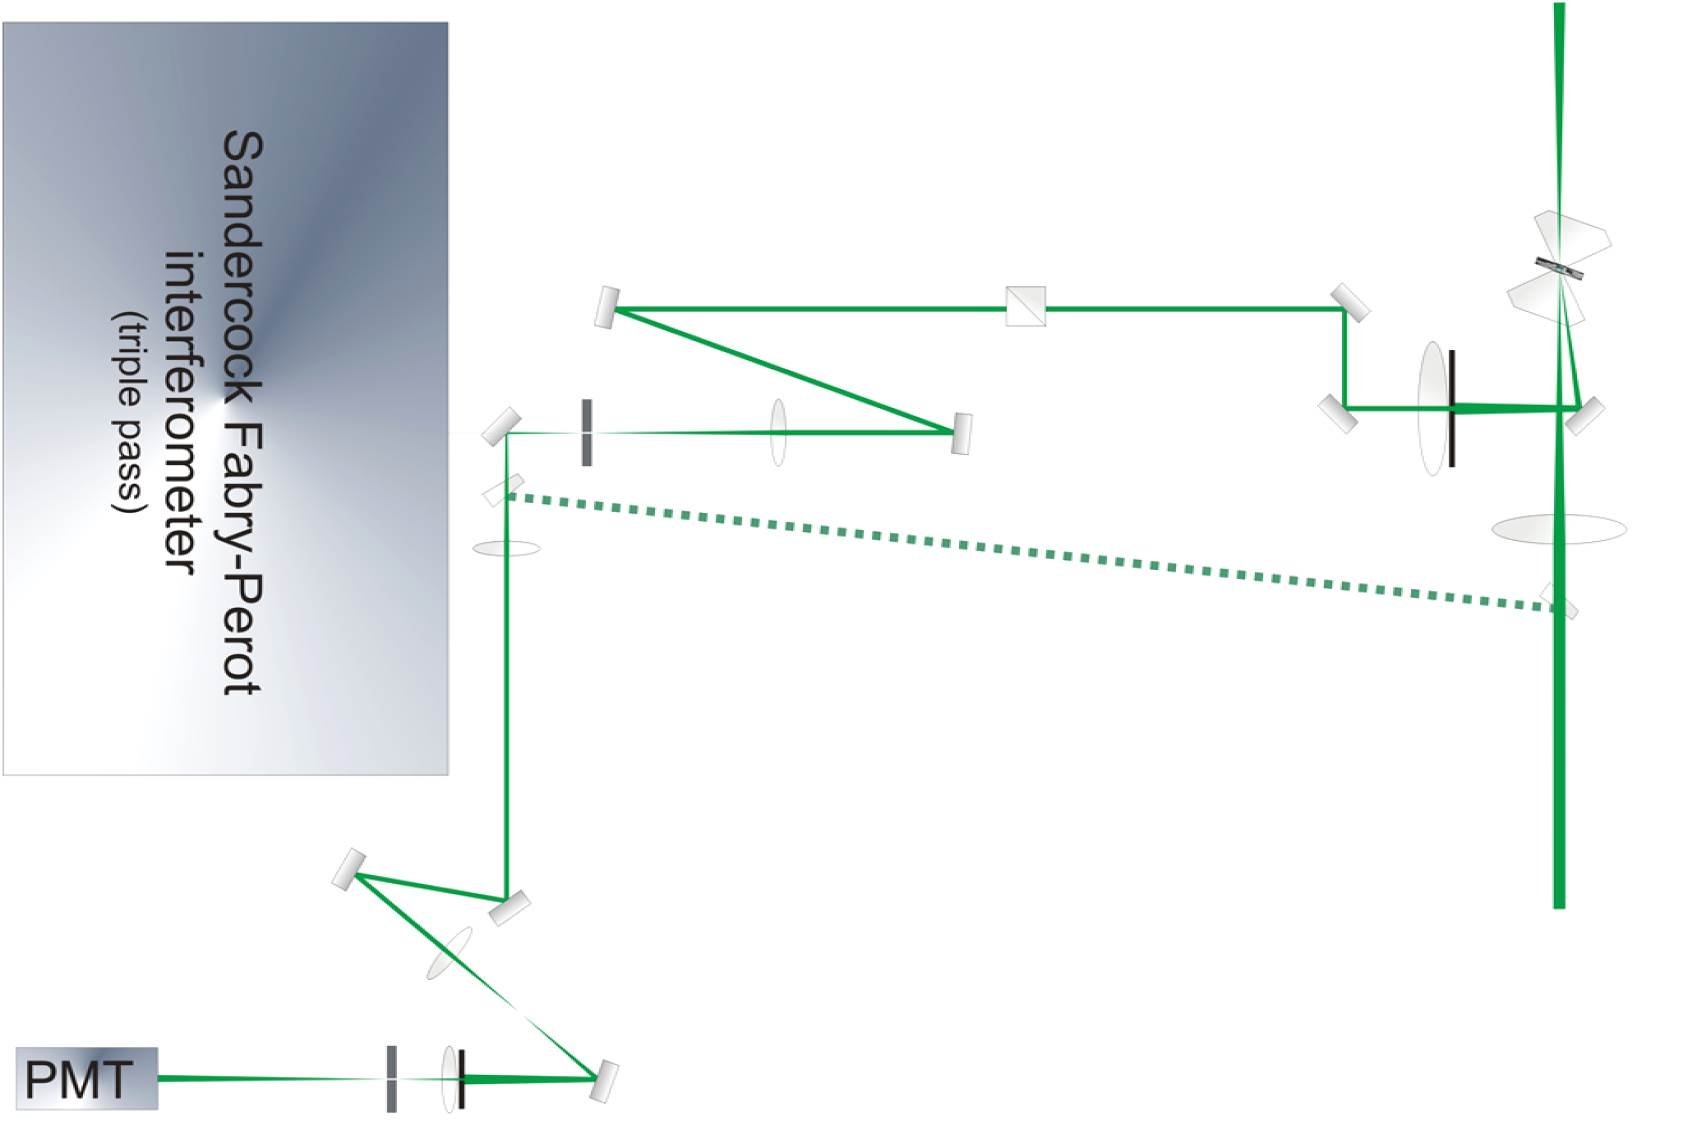
\includegraphics[width=\textwidth]{PCSsetup.jpg}};
		\node at (7.6,2.8) {a};
		\node at (7.6,1.2) {b};
		\node at (1.8,3.0) {c};
		\node at (-3.5,1.75) {d};
		\node at (-3.0,-4.2) {e};
	\end{tikzpicture}
	\caption{Major components of the experimental setup for DPCS: (a) DAC, (b) 1~cm mirror to redirect the scattered signal, (c) polarizer, (d) flip mirror to redirect the signal from the interferometer to the autocorrelator. The spectrum analyzer is a Sandercock-type tandem Fabry--P\'erot interferometer operated in a multi-pass (triple-pass tandem) configuration, corresponding to a total of six passes through the etalons, thereby providing substantially enhanced contrast and spectral resolution compared to a single- or double-pass design. Irises and pinholes are shown as black and gray bars, respectively. The dashed line represents a failed attempt to provide a local oscillator for heterodyne DPCS analysis.}
	\label{figure:PCSsetup}
\end{figure}
A Coherent Innova 306 actively locked single-mode Ar\textsuperscript{+} medium-frame laser operating at 514~nm provided the light source. To ensure the highest level of power stability, the laser was allowed to warm up at a set current near its operating point for one to two hours. At that stage, manual adjustments were made to the rear mirror to maximize output. Power and mode tracking were then enabled at 1~W output, and the laser was left to warm up for an additional half hour, with occasional alignment adjustments to minimize the operating current. Approximately once per week, the mode-tune algorithm was executed following this warm-up procedure.  

A set of reflective neutral-density filters allowed this 1~W output to be incrementally adjusted between 1 and approximately 30~mW while maintaining the power stability of the laser. Because the expected scattering signals are exceedingly weak, laser stability was of paramount importance. Future improvements to this system may include the implementation of cross-correlation, which would reduce dependence on power stability and enable analysis of even weaker scattering systems.

As shown in \fig \ref{figure:PCSsetup}, the beam is focused through the DAC located at position (a). The DAC is mounted on a four-axis stage that allows for $x$, $y$, $z$, and $\theta$ translations of the cell. What we will refer to as the $z$-axis is aligned along the incoming focused laser beam and is the primary axis that must be adjusted during signal optimization, as will be discussed shortly. The $\theta$ axis lies in the plane of the optical table and allows the DAC to be rotated as shown. In a typical Brillouin experiment, the DAC is rotated away from the collection mirror in order to reduce the amount of spectrally reflected light mixed with the desired signal.  

It should be noted that changes to $\theta$ do not affect the scattering vector $\vec{q}$, which is geometrically fixed by the collection mirror at location (b). This $1 \,\si{\centi\meter}$ diameter mirror is placed as close as possible to the incoming beam without occultation in order to closely approximate a 180\textdegree{} backscattering geometry. The external angle between the incoming beam and the path from the scattering volume to the center of the mirror is less than 3\textdegree. However, due to the indices of refraction of both the diamonds and the liquid sample, the actual scattering angle is significantly smaller—estimated to be less than 1\textdegree.  

The collimating optic that follows is preceded by an iris, which is used in Brillouin studies to restrict the scattering vector $\vec{q}$ collected. Here, however, the iris is opened reasonably wide but still serves to limit the collection cone, effectively providing a degree of low-resolution spatial filtering by rejecting off-axis light. The collimated light then passes through a polarizer at location (c), which may be removed for alignment purposes and replaced to select the depolarized component of the scattering signal. The beam height is then adjusted by the next two mirrors, placed intentionally after the polarizer, to match the input height of the interferometer. A $200 \,\si{\micro\meter}$ pinhole provides spatial filtering, and the flip mirror at location (d) is rotated out of the path of the incoming light to allow for spectral analysis.

\pgfplotsset{table/search path={Chapters/PCS/Figures}}
\begin{figure}[!htbp]
	\centering
	\begin{tikzpicture}
		\begin{axis}[
			ylabel={PMT counts},
			xlabel={Frequency (\si{\giga\hertz})},
			xmin=-15, xmax=15
			]
			\addplot table [only marks, x=a, y=b, col sep=comma] {BrillouinLA.csv};
		\end{axis}
	\end{tikzpicture}
	\caption{Typical Brillouin spectrum with the polarizer removed. The rapidly forming longitudinal acoustic (LA) peaks are used to optimize the DAC position for maximum signal. The polarizer is then reinserted and rotated until the LA peaks are suppressed, ideally leaving only the depolarized signal for DPCS analysis.}
	\label{figure:LAmodes}
\end{figure}

Even at relatively low pressures, far from the glass transition, light scattered from longitudinal acoustic modes gives rise to classic Brillouin peaks, as shown in \fig \ref{figure:LAmodes}. Here the spatial filtering may be optimized via maximizing the intensity of these longitudinal acoustic mode peaks. This is done predominately by adjusting the before-mentioned $z$-axis which translates the DAC along the path of the incoming laser light such that the collection area being focused onto the pinhole at location (d) corresponds to the liquid sample between the diamond culets. The fact that this Brillouin spectra forms significantly more quickly than the much weaker depolarized spectrum allows for rapid optimization of the spatial filtering. Once this is achieved, the polarizer is replaced and oriented to suppress the LA-modes—passing only the depolarized component of the scattered light. The mirror at location (d) is then flipped up, redirecting the spatially filtered light towards the autocorrelator PMT. The next focusing optic re-collimates the light after the pinhole and is followed by two mirrors to once again adjust the height of the beam to match the input height of the autocorrelator optics. The autocorrelator setup itself was previously designed for use with a 1cm cuvette and it was desirable not to strip the system of this capability. As such, the original PCS system was left intact so that a cuvette and oven could be placed at location (e) or removed at will. To accommodate for DPCS in the DAC, the lens following the height adjustment mirrors creates an image of the DAC sample at location (e) which the PCS setup then further spatially filters before directing the light to the PMT.  

\subsection{Homodyne \vs Heterodyne} \label{sec:HomoHeto}

As mentioned in \sect \ref{sec:PCSIntro}, DPCS may be performed in either a homodyne (self-beating) or a heterodyne (local oscillator) arrangement. What was not previously discussed is the requirement that one must be squarely within one of these two regimes in order to avoid prohibitively complex analysis. Elimination of the heterodyne component in the collected light signal is a significant hurdle when attempting PCS within a DAC. The surrounding structure, the edges of the gasket, every surface interface, and even inevitable dust on the diamond table scatter light with appreciable intensity. This problem is further exacerbated by the exceedingly small scattering volume (on the order of a nanoliter), making it easy for the heterodyne contribution to be comparable to—or even significantly stronger than—the light scattered from the sample volume.  

In depolarized studies, much of the heterodyne signal is immediately rejected by the polarizing prism. However, due to the finite extinction ratio of the polarizer a substantial component of the local oscillator inevitably bleeds through. Herbst \etal devoted considerable effort to addressing this challenge when first achieving PCS in a DAC\nolinebreak\cite{Herbst}. They were able to approach near-homodyne conditions through proper orientation of the DAC to deflect spectral reflections away from the collection optics, combined with spatial filtering of the collected light.

Their method, however, becomes increasingly difficult to apply when one wishes to directly probe density fluctuations in a pure liquid. Despite similar sample volumes, Herbst \etal measured the thermal diffusion of $\sim 90~\si{\nano\meter}$ polystyrene spheres and thus benefited from orders-of-magnitude greater scattering intensity. Even in this case, the heterodyne component was not fully eliminated and required careful alignment and modeling to minimize its influence. It is therefore not clear that, when scattering from density fluctuations in a pure liquid, near-homodyne conditions can be reliably maintained. Some amount of spectrally reflected light from gasket and diamond interfaces will likely be collected along with the desired signal, despite best efforts at spatial filtering. Future implementations may employ a Glan--Thompson polarizer, which offers extinction ratios on the order of $10^{5}$--$10^{6}$, significantly exceeding the $\sim 10^{3}$ typical of standard polarizing cubes, to more effectively suppress residual local oscillator contributions and thereby enable more robust homodyne conditions, mitigating the concerns discussed in the paragraphs that here follow.

A simple means to test whether conditions are reasonably within the heterodyne regime is to increase the intensity of the local oscillator and observe whether the extracted $\alpha$-relaxation times are affected. If the ratio of the local oscillator to the scattered signal can be increased significantly while the correlation function remains unchanged, then it is reasonable to infer that heterodyne conditions are being realized. An explicit heterodyne configuration, in which a dedicated local oscillator path was introduced (indicated by the dashed line in \fig\ref{figure:PCSsetup}), was attempted. However, this approach did not yield a measurable correlation signal, likely due to the excessive difference in optical path-length leading to instability in the phase difference between sample and local oscillator. 

\begin{figure}[!htbp]
	
	
	\begin{tikzpicture}
		
		% Left image
		\node[anchor=south west, inner sep=0] (img1) at (0,0)
		{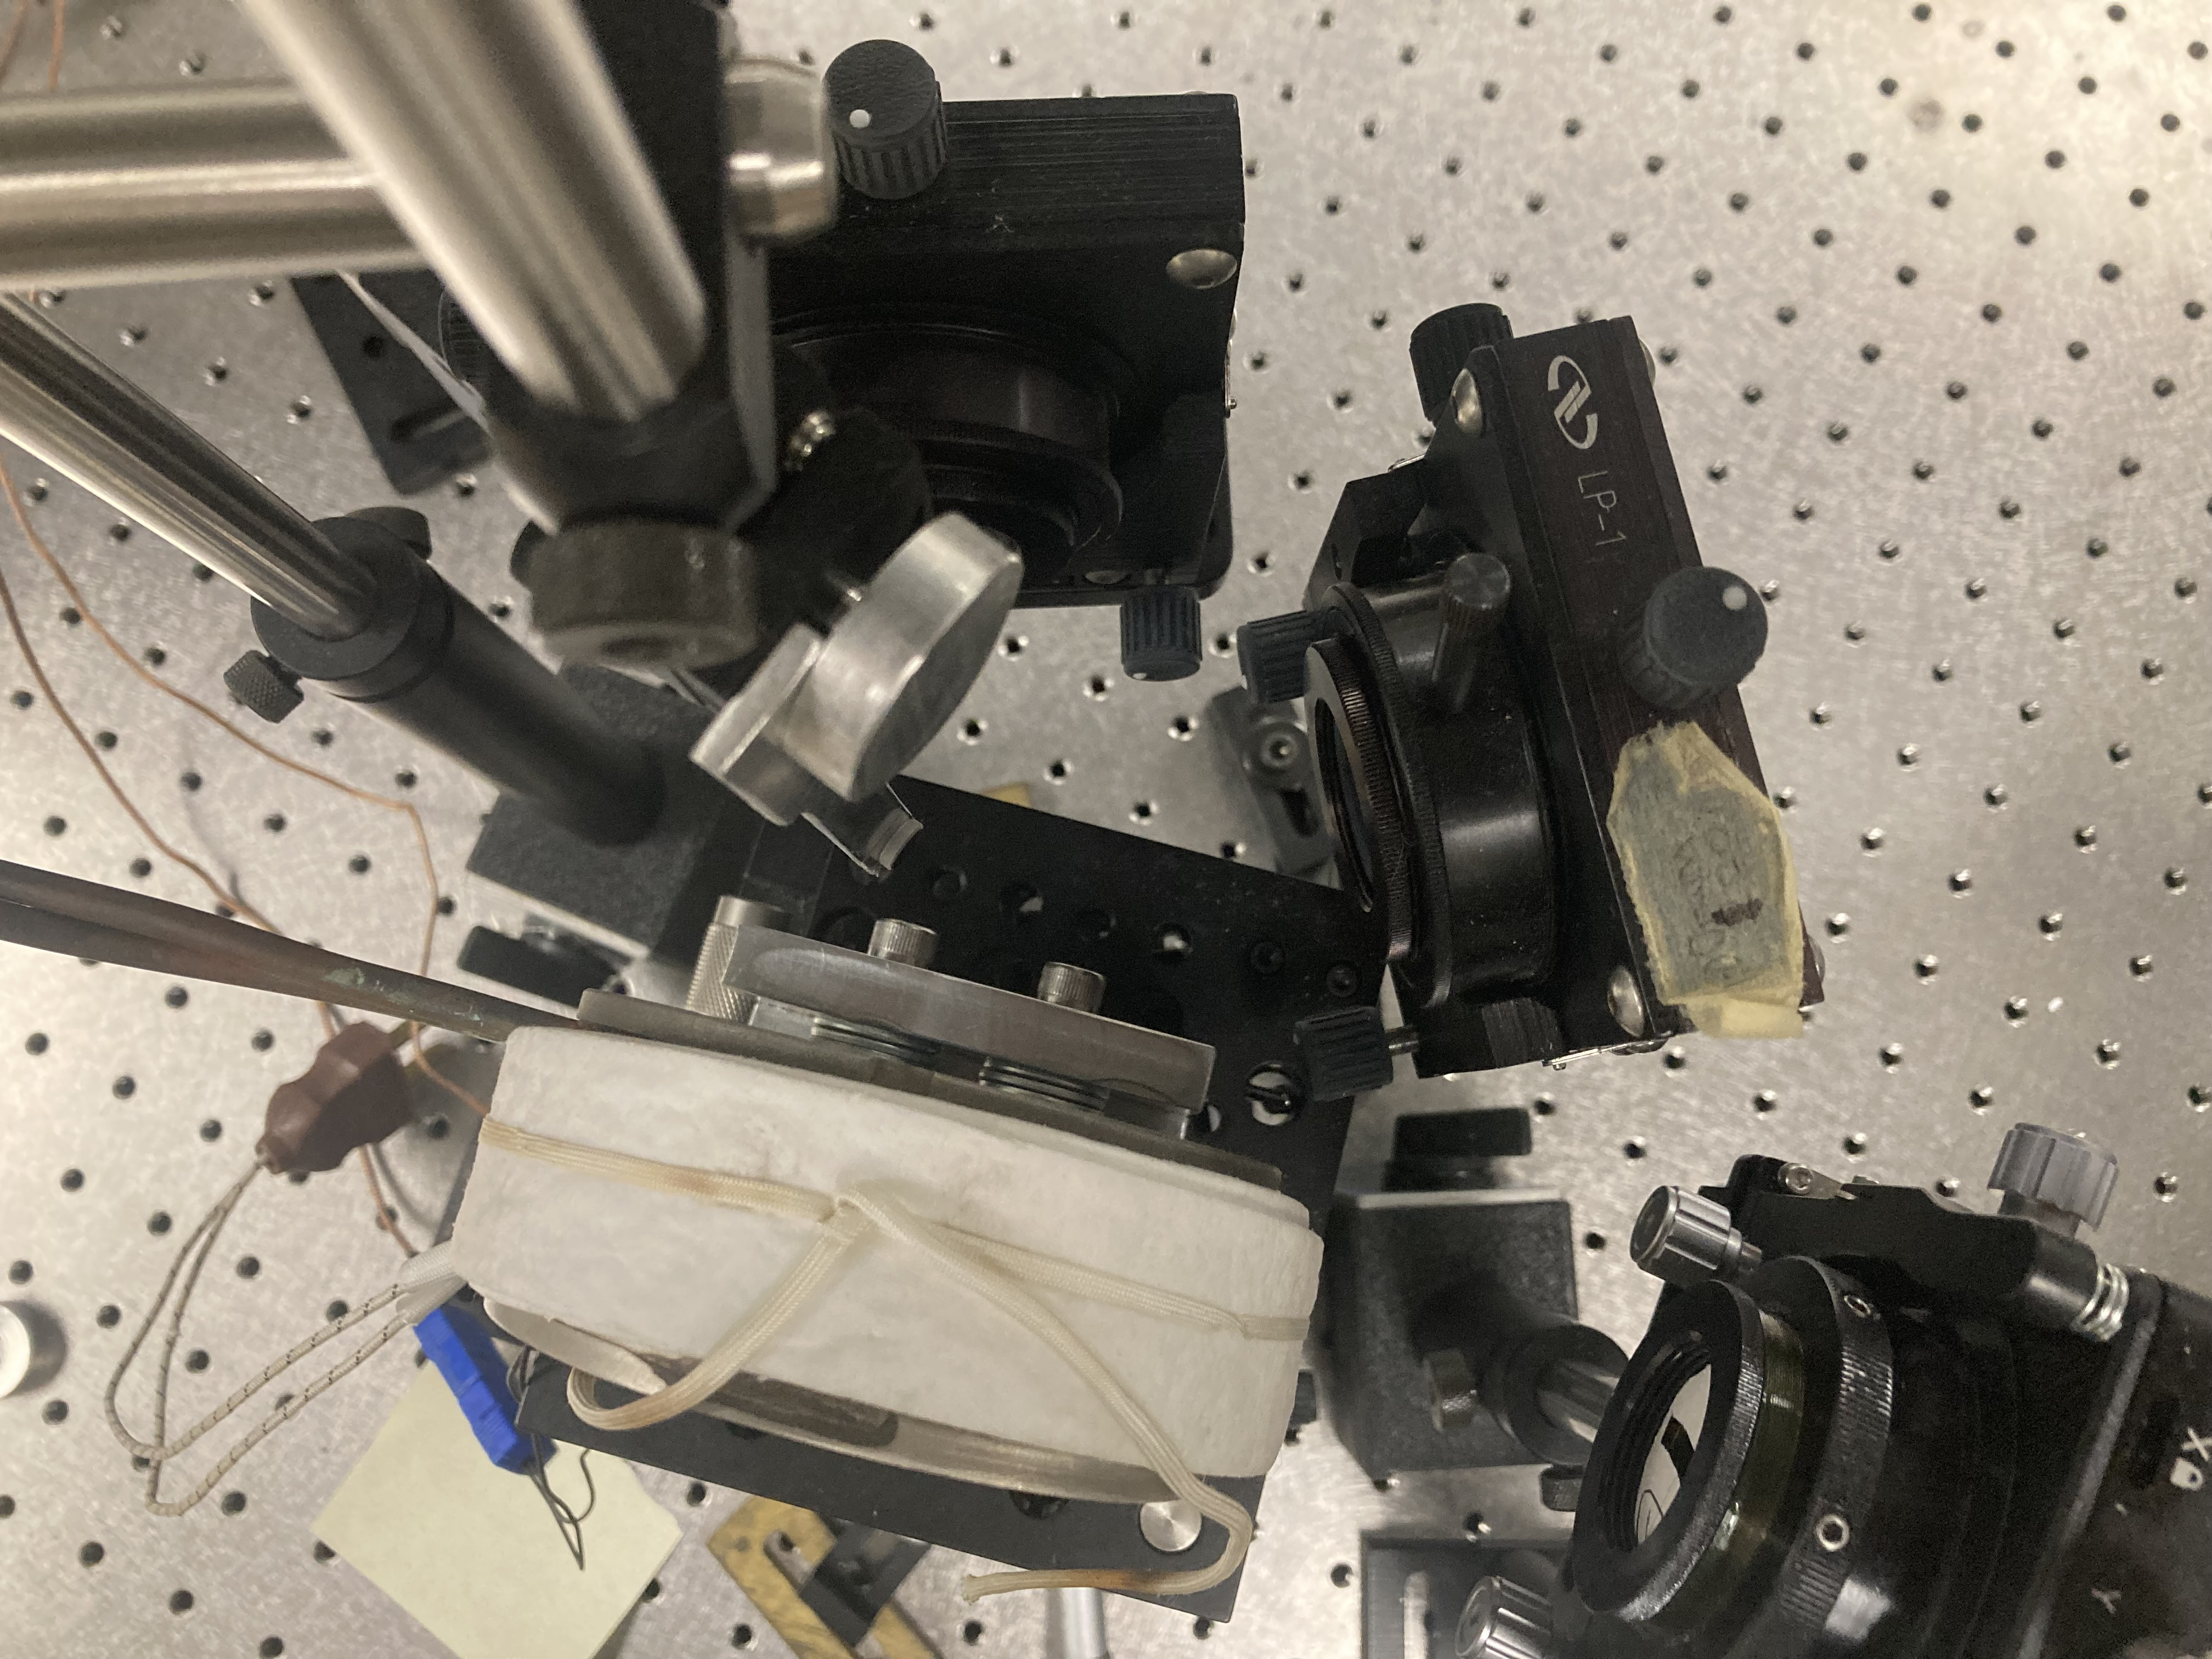
\includegraphics[width=0.45\textwidth]{IMG_1619.jpeg}};
		
		% Right image (shifted right)
		\node[anchor=south west, inner sep=0] (img2) at (0.5\textwidth,0)
		{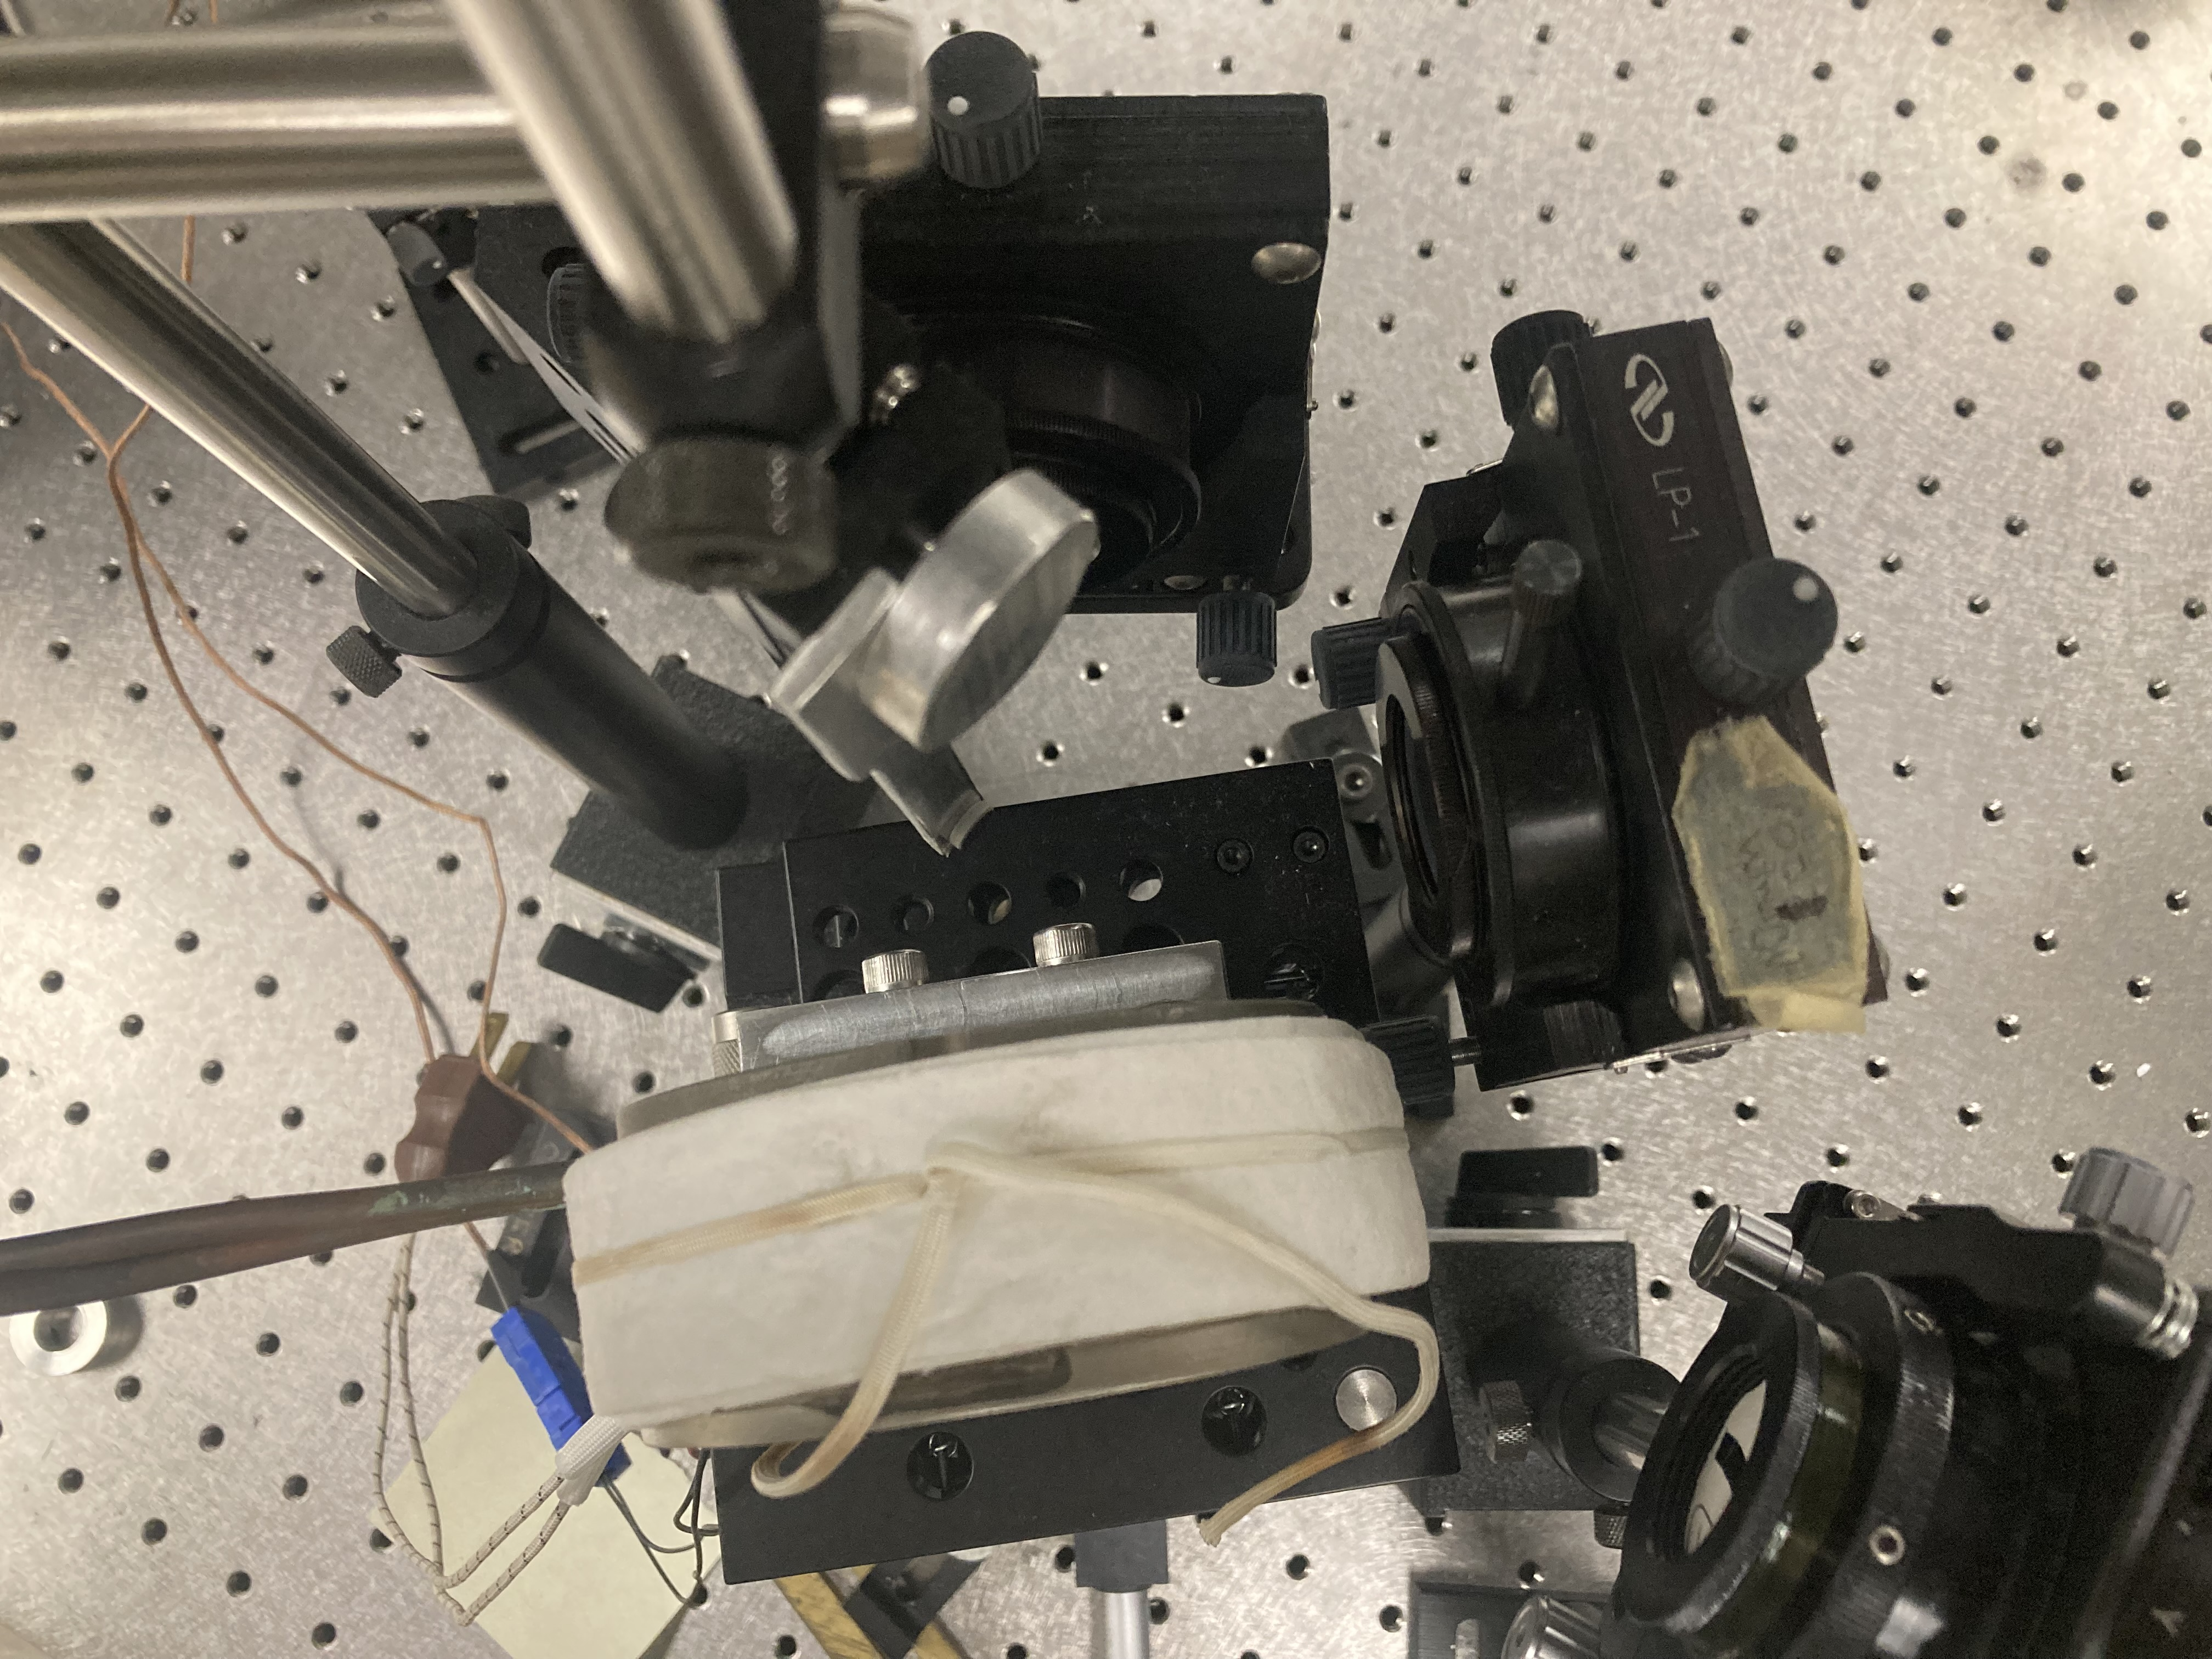
\includegraphics[width=0.45\textwidth]{IMG_1620.jpeg}};
		
		% Overlay for left image
		\begin{scope}[
			shift={(img1.south west)},
			x={($(img1.south east)-(img1.south west)$)},
			y={($(img1.north west)-(img1.south west)$)}
			]
			% draw on IMG_1619 here
			\draw[green, very thick,<-] (.42,0) -- (.42,1);
			\draw[green, thick] (.42,.25) -- (.41,.483);
			\draw[green, thick,->] (.41,.483) --(1,.6);
			
			\fill[green!60!black, opacity=0.25]
			(0.42,0.25) -- (0.6,1) -- (0.8,1) -- cycle;
			\draw[green!60!black, line width=0.5pt]
			(0.42,0.25) -- (0.6,1);
			\draw[green!60!black, line width=0.5pt]
			(0.42,0.25) -- (0.8,1);
			
			\node[red] at (0.2,0.45) {(BSM)};
			\draw[red,thick,->] (.28,.46) -- (.38,.481);
			
			\node[red] at (.32,0.25) {(DAC)};
			\node[red] at (.5,0.90) {(FO)};
			\node[red] at (.7,0.6) {(CO)};
		\end{scope}
		
		% Overlay for right image
		\begin{scope}[
			shift={($(img2.south west)+(0.25,0.08)$)},
			x={($(img2.south east)-(img2.south west)$)},
			y={($(img2.north west)-(img2.south west)$)}
			]
			
			% draw on IMG_1620 here
			\draw[green, very thick,<-] (.42,-0.01) -- (.42,.985);
			\draw[green, thick] (.42,.25) -- (.41,.483);
			\draw[green, thick,->] (.41,.483) --(.96,.6);
			
			\fill[green!60!black, opacity=0.25]
			(0.42,0.25) -- (0.2,.985) -- (0.4,.985) -- cycle;
			\draw[green!60!black, line width=0.5pt]
			(0.42,0.25) -- (0.2,.985);
			\draw[green!60!black, line width=0.5pt]
			(0.42,0.25) -- (0.4,.985);
		\end{scope}
		
	\end{tikzpicture}
	\caption{Optical geometry of the DAC assembly illustrating the role of specular reflections. In the left panel, the diamond anvil cell (DAC) is oriented to reject specular reflections from the diamond and gasket interfaces, minimizing the amount of reflected light collected by the detection optics. The shaded green conical region represents the angular distribution of this specular ``splash.'' The labeled components are the focusing optic (FO), collection optic (CO), back-scatter mirror (BSM), and diamond anvil cell (DAC). In the right panel, the DAC is intentionally rotated to direct this specular reflection onto the BSM, providing a local oscillator for heterodyne data acquisition.}
	\label{figure:DACStage}
\end{figure}

The solution was to invert the procedure of Herbst \etal: rather than rotating the DAC to reduce specular reflections, we incrementally rotated it to increase the amount of reflected light impinging on the collection optics, thereby providing a local oscillator of increasing intensity. The diamond anvil cell (DAC) is mounted on a precision translation and rotation stage, allowing for fine control of the scattering geometry. A representative view of the DAC mounted on the assembly stage is shown in \fig \ref{figure:DACStage}, illustrating the physical arrangement of the cell and the approximate scattering geometry used in this work.  

Successful heterodyne detection requires that the local oscillator and the scattered field traverse optical paths that are as nearly identical as practicable prior to mixing at the detector in order to assure a stable phase relationship. Utilizing spectrally reflected light from the diamond culets and gasket interfaces as the local oscillator naturally satisfies this requirement, as both the scattered and reflected fields originate within the same confined DAC geometry and propagate through essentially the same optical elements. Consequently, any difference in optical path length is limited to at most a small fraction of the culet separation ($\leq 100\,\si{\micro\meter}$), ensuring adequate phase coherence at the detector.  Correlation functions were obtained at a fixed pressure and temperature while incrementally increasing the angle subtended between the DAC and the incoming laser beam. The results are summarized in \tbl \ref{table:HetHomo}.  

\begin{table}[!htbp]
	\centering
	
	\tabletitle{PMT counts and relaxation times vs. DAC angle}
	\label{table:HetHomo}
	
	\begin{tabular}{lccc}
		\hline
		Angle (degrees) & Counts (thousands) & $\langle \tau \rangle$ ($\mu$s) & $\Delta \langle \tau \rangle$ ($\mu$s) \\
		\hline
		0  & 200 & 1360 & 54  \\
		5  & 164 & 1188 & 57  \\
		10 & 156 & 1296 & 73  \\
		15 & 120 & 1232 & 33  \\
		20 & 250 & 1449 & 57  \\
		\hline
	\end{tabular}
	
	\tabledescription{PMT count rates (in thousands) and corresponding $\alpha$-relaxation times $\langle \tau \rangle$ are shown as a function of DAC orientation. Zero degrees corresponds to the incoming laser at normal incidence to the diamond table; the DAC was then rotated \textit{toward} the collection mirror. The angular position was set using a calibrated rotation stage with an estimated uncertainty of $\pm 1^\circ$. The reported uncertainties $\Delta \langle \tau \rangle$ correspond to one-standard-deviation errors obtained from the covariance matrix of the nonlinear least-squares fits to the Cole--Davidson model.}
\end{table}

What is of primary interest here is how the expectation value of the relaxation time changes with increasing intensity of any heterodyne component. It is reasonable to assume that the intensity of light scattered directly from the sample is not substantially increased simply by rotating the DAC twenty degrees. Thus, the observed increase in PMT counts at certain angular positions must arise predominantly from additional scatter and specular reflections originating from the sources previously discussed.  

Although \fig \ref{figure:HetHomo} does appear to suggest an increasing trend in $\langle \tau \rangle$ as the heterodyne component is enhanced, it should be emphasized that the PMT counts more than double. As a bare minimum, then, the intensity of the local oscillator has been doubled, yet this corresponds to only a $\sim$17\% increase in $\langle \tau \rangle$. This outcome implies that the experiment is operating near, though perhaps not fully within, the heterodyne regime. We will later find the assumption that we are effectively within the heterodyne regime consistent with dynamic data obtained via other probes, including Brillouin scattering, \tgp, \etc

\begin{figure}[!htbp]
	\centering
	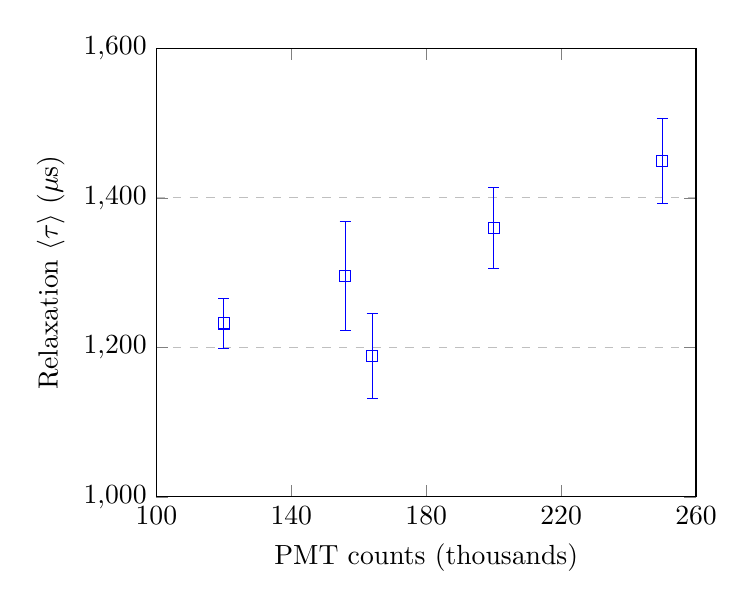
\begin{tikzpicture} 
		\begin{axis}[
			ylabel={Relaxation $\langle \tau \rangle$ ($\mu$s)},
			xlabel={PMT counts (thousands)},
			xmin=100, xmax=260,
			ymin=1000, ymax=1600,
			xtick={100,140,180,220,260},
			ytick={1000,1200,1400,1600},
			ymajorgrids=true,
			grid style=dashed,
			]
			\addplot+[only marks, mark=square, error bars/.cd, y dir=both, y explicit]
			coordinates { 
				(200,1360) +- (0,54) 
				(164,1188) +- (0,57) 
				(156,1296) +- (0,73) 
				(120,1232) +- (0,33) 
				(250,1449) +- (0,57) };
		\end{axis} 
	\end{tikzpicture}
	\caption{Structural relaxation times $\langle \tau \rangle$ as a function of increasing scatter and specular reflections serving as a local oscillator. Error bars represent 95\% confidence intervals derived from the mean square error (MSE) of the fit parameter $\tau$.}
	\label{figure:HetHomo}
\end{figure}

\subsection{Time-Correlation Functions}
\label{sec:TimeCorrelation}

The correlation spectra arising from the Brownian motion of mono-disperse colloidal spheres suspended in a liquid provide a useful point of reference from which to discuss our choice of time-correlation function adopted in this work. Consider the case of mono-disperse polystyrene spheres in methanol within the context of photon correlation spectroscopy experiments like those of Herbst \etal These spheres undergo diffusive motion in a relatively simple energy landscape. The resulting autocorrelation function exhibits a single-exponential decay, characterized by a well-defined relaxation time $\tau$ associated with translational diffusion.

By contrast, a typical glass-forming liquid exhibits a broad distribution of relaxation times. This distribution may arise from spatial heterogeneity, where different local environments relax at different rates, or from the presence of distinct relaxation modes within the system, and in practice may reflect a combination of both effects. Unlike the simple diffusive case described above, the corresponding time-correlation functions are no longer single exponential decays. Historically, these correlation data have been fit to the Kohlrausch--Williams--Watts (KWW) function \cite{Cardona2007,Williams}, which takes the form given in \eqn \ref{eqn:KWW}. When interpreted as a normalized time-correlation function, this may be written as
\begin{equation}
	C(t) = e^{-(t/\tau_{ww})^{\beta_{ww}}}, \quad 0 < \beta_{ww} \le 1.
	\label{eqn:KWWcorr}
\end{equation}
\noindent Here, $\tau_{ww}$ is a characteristic relaxation time and $\beta_{ww}$ quantifies the degree of stretching relative to a simple exponential decay.

In light scattering experiments, the fundamental observable is the dynamic structure factor $S(\vec q,\omega)$, which is related to the underlying correlation function through a Fourier transform:
\begin{equation}
	S(\vec q,\omega) = \mathscr{F}\!\left[ C(\vec q,t) \right].
	\label{eqn:SqwFromC}
\end{equation}
Thus, the spectral shape measured in frequency-domain techniques such as Brillouin light scattering reflects the frequency content of the relaxation dynamics encoded in $C(t)$. In time-domain techniques such as depolarized photon--correlation spectroscopy (DPCS), $C(t)$ is measured somewhat more directly.

The use of the KWW function to describe glassy systems is theoretically compelling for many reasons, not the least of which is that it captures the broad distribution of relaxation times characteristic of heterogeneous dynamics. Although often introduced in the context of dielectric spectroscopy—where the Laplace transform of the time derivative of $C(t)$ is related to the complex dielectric constant $\varepsilon^*$ as shown in \eqn \ref{eqn:delcTrans}—this reflects largely historical convention. Light scattering instead probes spatiotemporal fluctuations of the susceptibility tensor, $\delta\chi_{ij}(\mathbf r,t)$, which are directly related to fluctuations in the dielectric tensor. Consequently, both dielectric and light scattering measurements arise from the same underlying dielectric susceptibility tensor; however, light scattering probes the stochastic temporal evolution of its thermal fluctuations, whereas dielectric spectroscopy measures its response to an externally applied field:
\begin{equation}
	\frac{\varepsilon^{*} - \varepsilon_{\infty}}{\varepsilon_{0} - \varepsilon_{\infty}}
	= \mathscr{L}\!\left[ -\frac{\mathrm{d}C(t)}{\mathrm{d}t} \right]
	\label{eqn:delcTrans}
\end{equation}

Importantly, \eqn \ref{eqn:SqwFromC} and \eqn \ref{eqn:delcTrans} remain valid for arbitrary normalized relaxation functions, corresponding to any distribution of relaxation pathways and associated relaxation times\textemdash certainly including both KWW and Cole--Davidson forms described in \sect \ref{sec:models}. In the special case where $\beta = 1$, \eqn\ref{eqn:KWWcorr} reduces to a single exponential decay, corresponding to a Debye relaxation governed by a single characteristic timescale as with the Brownian motion of mono-disperse spherical particles in methanol studied by Herbst \etal \cite{Herbst}. Here the dynamics arise from random momentum transfer due to continual collisions with surrounding solvent molecules. Under these conditions, the system exhibits a well-defined relaxation time set by viscous dissipation and thermal fluctuations, leading to a correlation function characterized by a single timescale $\tau$. The corresponding dynamic structure factor of \eqn \ref{eqn:SqwFromC} then assumes the familiar Lorentzian form in frequency space,
\begin{equation}
	S(\vec q,\omega) \propto \frac{1}{1 + (\omega \tau)^2}.
	\label{eqn:debye_scattering}
\end{equation}

When working in frequency space, such as with Brillouin light scattering or dielectric frequency-response analysis, the relaxation dynamics of glass-forming systems are often described by functional forms such as the Cole--Davidson function of \eqn \ref{eqn:ColeDavidson} which, despite initial appearances, is closely analogous to \eqn \ref{eqn:KWW}. Both equations lend themselves well to fitting the structural relaxation dynamics of glass forming liquids.  In Brillouin light scattering, the spectral shape of the dynamic structure factor is often described phenomenologically by
\begin{equation}
	S(\vec q,\omega) \propto \Re\!\left[
	\left( \frac{1}{1 + i \omega \tau_{\mathrm{CD}}} \right)^{\beta_{\mathrm{CD}}}
	\right],
	\label{eqn:CD_Sqw}
\end{equation}
\noindent which, for $\beta_{\mathrm{CD}}=1$ reduces to 
\begin{equation}
	S(\vec q,\omega) \propto
	\Re\!\left[
	\frac{1}{1 + i \omega \tau}
	\right]
	=
	\frac{1}{1 + (\omega \tau)^2},
	\label{eqn:AlsoDebye}
\end{equation}
\noindent equivalent to \eqn \ref{eqn:debye_scattering} arising from the KWW model.

The equivalence of \eqn \ref{eqn:CD_Sqw} and \eqn \ref{eqn:KWWcorr} when both $\beta_{ww}=1$ and $\beta_{\mathrm{CD}}=1$ might suggest that the Cole--Davidson function is the Fourier transform of the KWW stretched exponential. It is not. Both functions may be interpreted as arising from a distribution of elementary relaxation processes, each independently describable by a simple exponential decay in the time domain. However, because they assume fundamentally different distribution functions, the extracted values of their respective $\tau$ and $\beta$ are not identical.

This discrepancy is not inconsequential, since multiple probes, operating in both the frequency and time domains, are required to track molecular dynamics in glass-forming systems across an enormous dynamic range. In this study, we would like to fit time domain DPCS data to a Cole--Davidson distribution to assure direct comparability with Brillouin data taken in the frequency regime. Lindsey and Patterson made this possible\nolinebreak\cite{Lindsey}\textemdash relating these two models by explicitly assuming that the KWW and Cole--Davidson functions arise from distributions of simple exponential decays, as follows:

\begin{equation}e^{-(t/\tau_{\mathrm{KWW}})^{\beta}}= \int_{0}^{\infty} e^{-t/\tau}\rho_{\mathrm{KWW}}(\tau)\mathrm{d}\tau
\end{equation}

\noindent and

\begin{equation}\left( \frac{1}{1+i\omega\tau_{\mathrm{CD}}} \right)^{\beta_{\mathrm{CD}}}= \int_{0}^{\infty} \frac{1}{\tau}\left( \frac{1}{1+i\omega\tau} \right)\rho_{\mathrm{CD}}(\tau)\mathrm{d}\tau.
	\label{eqn:distCD}
\end{equation}

A great deal of effort was devoted to solving for these distributions, $\rho_{\mathrm{CD}}$ and $\rho_{\mathrm{KWW}}$. Lindsey and Patterson provided an explicit form for $\rho_{\mathrm{CD}}(\tau)$, given by

\begin{equation}\label{eqn}\rho_{\mathrm{CD}}(\tau) =\frac{\sin(\pi \beta_{\mathrm{CD}})}{\pi}\left( \frac{\tau}{\tau_{\mathrm{CD}} - \tau} \right)^{\beta_{\mathrm{CD}}}.\end{equation}

\noindent This distribution, obtained from \eqn \ref{eqn:distCD} together with the normalization condition

\begin{equation}\int_{0}^{\infty} \frac{1}{\tau}\rho_{\mathrm{CD}}(\tau)\mathrm{d}\tau = 1,
\end{equation}

\noindent allows one to define the Cole–Davidson function in the time domain. Recall that $\rho_{\mathrm{CD}}(\tau)$ was derived under the assumption that the Cole–Davidson form corresponds to a distribution of simple Debye processes.  The Cole–Davidson function can be written in the time domain as

\begin{equation}
	\left( \frac{1}{1 + i \omega \tau_{\mathrm{CD}}} \right)^{\beta_{\mathrm{CD}}}= \mathscr{L}\left[ -\frac{\mathrm{d}}{\mathrm{d}t}\int_{0}^{\tau_{\mathrm{CD}}} \frac{1}{\tau}e^{-t/\tau}\rho_{\mathrm{CD}}(\tau)\mathrm{d}\tau \right].
\end{equation}

The work of Lindsey and Patterson has been available for four decades, yet it is clear why it became common practice to fit time-domain data to a KWW stretched exponential and then convert the parameters, rather than fitting directly to the Cole–Davidson distribution. Requiring a nonlinear fit routine to perform this integration would have been prohibitively resource-intensive on 1980s hardware. It remains nontrivial even today, though it can be recast into a form involving one- and two-parameter Gamma functions which, with the aid of modern lookup tables, can be evaluated relatively efficiently as follows in \eqn \ref{eqn:timeColeDavidson}.

\begin{equation}
	\int_{0}^{\tau_{\mathrm{CD}}} \frac{1}{\tau}e^{-t/\tau}\rho_{\mathrm{CD}}(\tau)\mathrm{d}\tau= \frac{1}{\pi}\Gamma\left(1-\beta_{\mathrm{CD}}\right)\Gamma\left(\beta_{\mathrm{CD}}, \tfrac{t}{\tau_{\mathrm{CD}}}\right)\sin\left(\pi\beta_{\mathrm{CD}}\right)
	\label{eqn:timeColeDavidson}
\end{equation}

Thus, in order to obtain values of $\tau$ that are directly comparable to those derived from frequency-domain Brillouin studies, all DPCS time-domain correlation decays will be fit in \textit{Mathematica} to a distribution of single-exponential decays corresponding to a Cole–Davidson function in the frequency domain, as expressed in \eqn \ref{eqn:DPCS}.

\begin{equation}
	C_{\mathrm{CD}}(t) =\frac{1}{\pi}\Gamma\left(1-\beta_{\mathrm{CD}}\right)\Gamma\left(\beta_{\mathrm{CD}}, \tfrac{t}{\tau_{\mathrm{CD}}}\right)\sin\left(\pi \beta_{\mathrm{CD}}\right)
	\label{eqn:DPCS}
	\end{equation}

\section{Autocorrelation Data Analysis and Fitting Methodology}
\label{sec:DAC75CExample}

The sequence of experimentally determined autocorrelation functions presented in \fig \ref{fig:PCS75CRegression} is taken from the 75~\textdegree C isothermal cumene data covering a pressure range from 20.0 to 27.8 kbar, over which the structural relaxation time fits within the eight- to nine-decade time window of PCS. As noted previously in \sect \ref{sec:PCSExp}, autocorrelations obtained in a DAC are not expected to be as tidy as those from conventional cuvette geometries. Two experimental realities dominate the appearance of these data. First, microscopic impurities, gasket scatter, and dust create significant background scattering not associated with the liquid dynamics. At lower temperatures (or higher pressures) these larger scatterers are effectively immobile on our timescales and, along with spectral reflections, will tend the experiment towards the heterodyne regime. Under thermodynamic conditions for which $\tau_\alpha$ is sufficiently small, some of these particles become mobile on experimental timescales. When such a particle enters or leaves the scattering volume mid-acquisition, the baseline of the autocorrelation can swing substantially and may take impractically long to average back to a flat baseline.

\begin{figure}[!htbp]
	\centering
	\begin{tikzpicture}
		\begin{axis}[
			xlabel={Seconds},
			ylabel={Normalized Autocorrelation [$g_{2}(t)$]},
			title={\shortstack{Depolarized Photon Correlation Spectroscopy \\of Cumene at 75 °C}},
			grid=both,
			xmode=log,     
			xticklabel style={rotate=45, anchor=east}, 
			transpose legend,       
			legend pos=north east,
			legend columns=5,
			width=12cm, height=8cm
			]
			
			% 20.0 kbar (blue filled)
			\addplot[only marks, mark=*, mark size=1pt, color=blue, fill=blue] 
			table[col sep=comma, x={20_0kbar xd}, y={20_0kbar yd}] {Chapters/PCS/Figures/data.csv};
			\addlegendentry{\SI{20.0}{\kilo\bar}}
			\addplot[semithick, color=red, forget plot]
			table[col sep=comma, x={20_0kbar xf}, y={20_0kbar yf}] {Chapters/PCS/Figures/data.csv};
			
			% 21.5 kbar (orange open)
			\addplot[only marks, mark=o, mark size=1pt, color=orange] 
			table[col sep=comma, x={21_21kbar xd}, y={21_21kbar yd}] {Chapters/PCS/Figures/data.csv};
			\addlegendentry{\SI{21.5}{\kilo\bar}}
			\addplot[semithick, color=red, forget plot]
			table[col sep=comma, x={21_21kbar xf}, y={21_21kbar yf}] {Chapters/PCS/Figures/data.csv};
			
			% 22.1 kbar (green filled)
			\addplot[only marks, mark=triangle*, mark size=1.2pt, color=green, fill=green] 
			table[col sep=comma, x={22_06kbar xd}, y={22_06kbar yd}] {Chapters/PCS/Figures/data.csv};
			\addlegendentry{\SI{22.1}{\kilo\bar}}
			\addplot[semithick, color=red, forget plot]
			table[col sep=comma, x={22_06kbar xf}, y={22_06kbar yf}] {Chapters/PCS/Figures/data.csv};
			
			% 23.1 kbar (purple open)
			\addplot[only marks, mark=triangle, mark size=1.2pt, color=purple] 
			table[col sep=comma, x={23_14kbar xd}, y={23_14kbar yd}] {Chapters/PCS/Figures/data.csv};
			\addlegendentry{\SI{23.1}{\kilo\bar}}
			\addplot[semithick, color=red, forget plot]
			table[col sep=comma, x={23_14kbar xf}, y={23_14kbar yf}] {Chapters/PCS/Figures/data.csv};
			
			% 24.0 kbar (black open)
			\addplot[only marks, mark=square, mark size=1pt, color=teal] 
			table[col sep=comma, x={24_0kbar xd}, y={24_0kbar yd}] {Chapters/PCS/Figures/data.csv};
			\addlegendentry{\SI{24.0}{\kilo\bar}}
			\addplot[semithick, color=red, forget plot]
			table[col sep=comma, x={24_0kbar xf}, y={24_0kbar yf}] {Chapters/PCS/Figures/data.csv};
			
			% 24.9 kbar (blue filled again — cycle restarts)
			\addplot[only marks, mark=diamond*, mark size=1.2pt, color=blue, fill=blue] 
			table[col sep=comma, x={24_92kbar xd}, y={24_92kbar yd}] {Chapters/PCS/Figures/data.csv};
			\addlegendentry{\SI{24.9}{\kilo\bar}}
			\addplot[semithick, color=red, forget plot]
			table[col sep=comma, x={24_92kbar xf}, y={24_92kbar yf}] {Chapters/PCS/Figures/data.csv};
			
			% 25.2 kbar (orange open again)
			\addplot[only marks, mark=diamond, mark size=1.2pt, color=orange] 
			table[col sep=comma, x={25_2kbar xd}, y={25_2kbar yd}] {Chapters/PCS/Figures/data.csv};
			\addlegendentry{\SI{25.2}{\kilo\bar}}
			\addplot[semithick, color=red, forget plot]
			table[col sep=comma, x={25_2kbar xf}, y={25_2kbar yf}] {Chapters/PCS/Figures/data.csv};
			
			% 26.4 kbar (green filled again)
			\addplot[only marks, mark=pentagon*, mark size=1.3pt, color=green, fill=green] 
			table[col sep=comma, x={26_43kbar xd}, y={26_43kbar yd}] {Chapters/PCS/Figures/data.csv};
			\addlegendentry{\SI{26.4}{\kilo\bar}}
			\addplot[semithick, color=red, forget plot]
			table[col sep=comma, x={26_43kbar xf}, y={26_43kbar yf}] {Chapters/PCS/Figures/data.csv};
			
			% 26.8 kbar (purple open again)
			\addplot[only marks, mark=pentagon, mark size=1.3pt, color=purple] 
			table[col sep=comma, x={26_8kbar xd}, y={26_8kbar yd}] {Chapters/PCS/Figures/data.csv};
			\addlegendentry{\SI{26.8}{\kilo\bar}}
			\addplot[semithick, color=red, forget plot]
			table[col sep=comma, x={26_8kbar xf}, y={26_8kbar yf}] {Chapters/PCS/Figures/data.csv};
			
			% 27.8 kbar (teal filled again)
			\addplot[only marks, mark=star, mark size=1.3pt, color=teal, fill=teal] 
			table[col sep=comma, x={27_8kbar xd}, y={27_8kbar yd}] {Chapters/PCS/Figures/data.csv};
			\addlegendentry{\SI{27.8}{\kilo\bar}}
			\addplot[semithick, color=red, forget plot]
			table[col sep=comma, x={27_8kbar xf}, y={27_8kbar yf}] {Chapters/PCS/Figures/data.csv};
			
		\end{axis}
	\end{tikzpicture}
	\caption{DPCS autocorrelations of cumene measured in a DAC at 75~\textdegree C across a range of pressures over which $\tau_\alpha$ fits within the time window of our autocorrelator. The sequence highlights two dominant elevated-temperature artifacts: slowly varying baseline offsets and photon-limited short-lag noise. Mitigation and fitting strategy are discussed in the text.}
	\label{fig:PCS75CRegression}
\end{figure}

This fluctuating baseline is shown in \fig \ref{fig:PCS75CBaseline} for one of our higher-pressure datapoints\textemdash 26.8 kbar. It should be noted that these are not taken at set time intervals but are instead the result of periodically saving the acquisitions during long runs; one never knows when a severe baseline fluctuation may render the data unfittable, so earlier saved autocorrelations can preserve a data point that often required hours, if not days, to obtain.

It may also be seen from \fig \ref{fig:PCS75CBaseline} that the first autocorrelation was saved relatively early, before the decay had fully converged to the actual relaxation\textemdash \ie, it lies well above the regressions saved at later times. However, all of the subsequent regressions quickly converge, as was typical for all acquisitions, even though the baseline at high pressures and temperatures very rarely does so for the aforementioned reasons.


\begin{figure}[!htbp]
	\centering
	\begin{tikzpicture}
		\begin{axis}[
			xlabel={Seconds},
			ylabel={Normalized Autocorrelation [$g_{2}(t)$]},
			title={Baseline Instability in DAC for Cumene at 75 °C},
			grid=both,
			xmode=log,     
			xticklabel style={rotate=45, anchor=east}, 
			transpose legend, 
			legend cell align=left,      
			legend pos=north east,
			legend columns=1,
			width=12cm, height=8cm
			]
			
			% t=1
			\addplot[only marks, mark=*, mark size=1pt, color=gray, fill=gray] 
			table[col sep=comma, x={x15nv04_1}, y={y15nv04_1}] {Chapters/PCS/Figures/data.csv};
			\addlegendentry{First};
			
			% t=2
			\addplot[only marks, mark=o, mark size=1pt, color=orange, fill=orange] 
			table[col sep=comma, x={x15nv04_2}, y={y15nv04_2}] {Chapters/PCS/Figures/data.csv};
			\addlegendentry{Second};
			
			% t=3
			\addplot[only marks, mark=triangle*, mark size=1pt, color=green, fill=green] 
			table[col sep=comma, x={x15nv04_3}, y={y15nv04_3}] {Chapters/PCS/Figures/data.csv};
			\addlegendentry{Third};
			
			% t=4
			\addplot[only marks, mark=triangle*, mark size=1pt, color=purple, fill=purple] 
			table[col sep=comma, x={x15nv04_4}, y={y15nv04_4}] {Chapters/PCS/Figures/data.csv};
			\addlegendentry{Fourth};
			
			% t=5
			\addplot[only marks, mark=square, mark size=1pt, color=teal, fill=teal] 
			table[col sep=comma, x={x15nv04_5}, y={y15nv04_5}] {Chapters/PCS/Figures/data.csv};
			\addlegendentry{Fifth};
			
			% t=6
			\addplot[only marks, mark=diamond*, mark size=1pt, color=blue, fill=blue] 
			table[col sep=comma, x={x15nv04_6}, y={y15nv04_6}] {Chapters/PCS/Figures/data.csv};
			\addlegendentry{Sixth};
					
		\end{axis}
	\end{tikzpicture}
	\caption{Autocorrelations of cumene at 75~\textdegree C and $26.8$ kbar illustrating the fluctuating baselines characteristic of DAC measurements under thermodynamic conditions such that mobile contaminants interfere with data analysis. Each curve represents a saved acquisition taken at a different time during the run. The earliest save (``First'') was recorded before the decay had fully converged to the true relaxation and therefore lies well above the later regressions. Subsequent saves converge rapidly to a consistent relaxation profile, while the overall baseline remains unstable likely due to mobile impurities entering or leaving the scattering volume mid-acquisition.}
	
	\label{fig:PCS75CBaseline}
\end{figure}

An additional consideration is that the DAC severely limits the illuminated/scattering volume. Scattering volumes typical for PCS in a cuvette are often on the order of hundreds of nanoliters. However, because the culets of the DAC constrain the length of the scattering column, often to 100 microns or less, the effective scattering volume may be reduced by two orders of magnitude or more to that which is common in a more classical cuvette-centered experimental setup. For the fastest autocorrelation channels this often implies $\ll 1$ photon per scan on average, so the short-lag-time ``head'' of the normalized autocorrelation function $g_{2}(t)$ is photon-shot-noise dominated. This gives rise to the poorly defined low-lag region shown in \fig \ref{fig:PCS75CHead}. Unlike baseline drift, this head noise persists even at relatively low temperatures or high pressures, as it originates from photon statistics within a tiny scattering volume. At lower temperatures or higher pressures, however, the intrinsic dynamics are much slower, and the shot noise inherent to these fast channels becomes of little consequence. In fact, it is quite common for the autocorrelation curve to lack a head entirely at high temperatures or low pressures where the liquid's structural relaxation time lies beyond or just outside the range of the correlator's fastest channels. This behavior is clearly visible in the data presented in \fig \ref{fig:PCS75CRegression}, taken at 22.1 kbar and 75~\textdegree C.

 
\begin{figure}[!htbp]
	\centering
	\begin{tikzpicture}
		\begin{axis}[
			xlabel={Seconds},
			ylabel={Normalized Autocorrelation [$g_{2}(t)$]},
			title={\shortstack{Photon Shot-Noise--Dominated Short-Lag Region\\in DAC for Cumene at 75 °C}},
			grid=both,
			xmode=log,     
			xticklabel style={rotate=45, anchor=east}, 
			xmax=.01,
			transpose legend,  
			legend cell align=left,      
			legend pos=north east,
			legend columns=1,
			width=12cm, height=8cm
			]
			
			\addplot[only marks, mark=*, mark size=1pt, color=blue, fill=blue] 
			table[col sep=comma, x={22_06kbar xd}, y={22_06kbar yd}] {Chapters/PCS/Figures/data.csv};
			\addlegendentry{\SI{22.1}{\kilo\bar}}
			
			\addplot[mark=none, color=red] 
			table[col sep=comma, x={22_06kbar xf}, y={22_06kbar yf}] {Chapters/PCS/Figures/data.csv};
			\addlegendentry{Cole-Davidson fit}
			
		\end{axis}
	\end{tikzpicture}
	\caption{Autocorrelation of cumene at 75\textdegree C and \SI{22.1}{\kilo\bar} illustrating the shot-noise–dominated short-lag region that arises from the severely reduced scattering volume in the DAC.}
	
	
	\label{fig:PCS75CHead}
\end{figure}

Despite these complications being more pronounced at higher temperatures, the 75~\textdegree C data series is included here as it represents the “worst-case’’ data quality we encountered and thus motivates the regression fit strategy outlined below which has been implemented here to extract reliable relaxation times.

Obtaining robust Cole–Davidson fits in the time domain ideally requires well-defined heads and baselines. Of these, the baseline is often most critical given that, for the Cole-Davidson distribution, $\tau_{\mathrm{CD}}$ is the discrete upper cutoff of the structural-relaxation mode distribution. The expectation value satisfies $\langle \tau \rangle_{\mathrm{CD}}=\beta_{\mathrm{CD}}\,\tau_{\mathrm{CD}}$. In the DAC, especially at higher temperatures, a clean baseline can be unattainable, while at the fastest lags the head can be too noisy to anchor the early-time curvature due to shot noise. The practical remedy is therefore to constrain the shape parameter, $\beta_{\mathrm{CD}}$, or at least to establish a functional dependence of $\beta_{\mathrm{CD}}$ on pressure and temperature. Without such a constraint, the fit becomes underdetermined when either the head or baseline is unreliable. When a portion of the autocorrelation function must be excluded, whether the early-time head or the late-time baseline, fixing $\beta_{\mathrm{CD}}$ removes the principal degeneracy between amplitude and shape in the fit. This constraint allows $\tau_{\mathrm{CD}}$ to be determined primarily by the curvature of the mid-lag region. In practice, most datasets furnish at least one clean side, so constraining $\beta_{\mathrm{CD}}$ empirically or through a pressure-temperature-dependent model would ensure consistent $\tau_{\mathrm{CD}}$ values and hence consistent mean relaxation times $\langle \tau \rangle = \beta_{\mathrm{CD}}\tau_{\mathrm{CD}}$.

\begin{figure}[!htbp]
	\centering
	\begin{tikzpicture}
		\node[anchor=south west, inner sep=0] (img) at (0,0)
		{
\includegraphics[width=0.85\linewidth]{chapters/pcs/figures/Beta Analysis.JPG}};
		
		\begin{scope}[
			x={($(img.south east)-(img.south west)$)},
			y={($(img.north west)-(img.south west)$)}
			]
			% Cover old "DLS" label
			\fill[white] (0.835,0.35) rectangle (0.955,0.45);
			
			% Write corrected labels
			\node[anchor=west] at (0.835,0.425) {\fontsize{12}{11}\selectfont DBLS};
			\node[anchor=west] at (0.835,0.38) {\fontsize{12}{11}\selectfont DPCS};
		\end{scope}
	\end{tikzpicture}
	\caption{Pressure dependence of the Cole--Davidson shape parameter, $\beta_{\mathrm{CD}}$, obtained from depolarized Brillouin (black circles) and DPCS (green diamonds) measurements. Error bars represent $1\sigma$ uncertainties derived from the nonlinear fit covariance matrices. The inset shows the temperature dependence of $\beta_{\mathrm{CD}}$ at selected pressures, demonstrating its statistical invariance across a large experimental domain.}
	\label{fig:beta}
\end{figure}

As it happens, our lab has plenty of relaxation data at various pressures and temperatures for cumene in the form of depolarized Brillouin light-scattering data as well as DPCS.  The values for $\beta_{\mathrm{CD}}$ along with $1\sigma$ uncertainties derived from the covariance matrix of the nonlinear fits, is shown in \fig \ref{fig:beta}.  It is notable that the error bars for $\beta_{\mathrm{CD}}$ become excessively large near ambient pressure.  The larger uncertainties in the Brillouin fits at low pressure arise due to the structural–relaxation (Mountain) component becoming less distinct from the quasi-elastic background near the Bose peak, increasing parameter covariance in the Cole–Davidson fits.  However, as there was no evident trend in the value of $\beta_{\mathrm{CD}}$ approaching the Bose peak, there is no reason to believe such a trend would suddenly appear as we approach ambient pressure.  To extend this analysis, DPCS data was also included under conditions where an autocorrelation could be obtained having a solid low-lag head and baseline thus allowing for a nonlinear fit from which $\beta_{\mathrm{CD}}$ could be confidently obtained.  This is particularly compelling as it not only extends our analysis of the pressure dependence of $\beta_{\mathrm{CD}}$ up to nearly $2.5~\si{\giga\pascal}$, but also further assures us that our time-domain Cole-Davidson fits to our autocorrelations are returning the appropriate values for comparison with our frequency-domain data.  It is very evident that there is no significant pressure dependence in the value of $\beta_{\mathrm{CD}}$ from ambient pressure up to nearly $2.5~\si{\giga\pascal}$.

The inset plot of \fig \ref{fig:beta} is comprised entirely of DPCS autocorrelation fits where solid low-lag heads and baselines were obtainable.  It is clear that over the range of 40~$^\circ$C for which these data were obtained there is no significant temperature dependence in the value of  $\beta_{\mathrm{CD}}$.  Thus, we make the assumption that, for the glass former cumene, over the ranges of pressure and temperature here investigated, the value of  $\beta_{\mathrm{CD}}=0.509$.  This value is used consistently for all Cole-Davidson fits to cumene data here presented.

For internal validation, we applied this procedure to runs where both a clean head and a flat baseline are present. The full autocorrelation is first fit with $\{\tau_{\mathrm{CD}},\beta_{\mathrm{CD}}\}$ free to obtain $\tau_{\mathrm{CD}}^{(\text{full})}$ and $\beta_{\mathrm{CD}}^{(\text{full})}$. The analysis is then repeated twice: once with the short-lag head removed and $\beta_{\mathrm{CD}}=0.509$, and once with the baseline removed and the same fixed $\beta_{\mathrm{CD}}$. In both cases the recovered $\tau_{\mathrm{CD}}$ agrees with $\tau_{\mathrm{CD}}^{(\text{full})}$ within the 95\% confidence interval, indicating that a single reliable side of the decay suffices when $\beta_{\mathrm{CD}}$ is constrained. 


\section{Results and Discussion}\label{sec:result}
\subsection{Thermodynamic Scaling}\label{sec:tdscaling}

Another means of validating the DPCS data—and of confirming that the measurements were obtained under heterodyne or homodyne experimental conditions—is to examine how well they conform to the established thermodynamic scaling behavior of cumene \cite{RansomPRL}. The cumene \tgp data, provided here and in \app \ref{app:CumeneIGP}, allows us to determine the appropriate scaling factor.  

Liquids that obey thermodynamic scaling exhibit a relationship between temperature, volume, and relaxation time of the form:  
\begin{equation}\label{eqn:tdscaling}
	\tau \propto \frac{1}{T V^{\gamma}}
\end{equation}

\noindent Experimentally, the \tgp process provides the glass-transition temperature as a function of pressure. To proceed, it is necessary to convert these pressures to the corresponding specific volumes. For cumene, this conversion is carried out using the modified Tait equation of state provided in \app \ref{app:CumeneEOS}.  

Thus, since the \tgp data comprise an isochronous curve at $\tau \approx 100 \,\si{\second}$, taking the logarithm of both sides of \eqn \ref{eqn:tdscaling} yields the linear expression in \eqn \ref{eqn:lingamma}. The slope of this relation gives the scaling factor $\gamma$, while the $y$-intercept provides an estimate of the relaxation time associated with the \tgp data.  

\begin{equation}\label{eqn:lingamma}
	\log_{10}(T) = -\gamma \log_{10}(V) - \log_{10}(\tau_{G})
\end{equation}

\noindent The TGP data for cumene from \app \ref{app:CumeneIGP} are plotted as $\log_{10}(T_g)$ versus $\log_{10}(V_g)$ and indeed our data show a very linear relation.  A linear regression yields a value of the scaling exponent for cumene of 4.77 and an intercept of 2.11, from which we calculate an average relaxation time of tau = 130 s for Tg(P).

\begin{figure}[!htbp]
	\centering
	\begin{tikzpicture} 
		\begin{axis}[
			title={Scaling Parameter from \tgp Data},
			ylabel={$\log_{10} T_{G}$},
			xlabel={-$\log_{10} V_{G}$},
			ymin=2.1, ymax=2.7,
			xmin=0, xmax=0.12,
			xtick={0,0.04,0.08,0.12},
			ytick={2.1,2.3,2.5,2.7},
			]
			\addplot table [only marks, x=a, y=b, col sep=comma] {TDScaling.csv};
			\addplot {4.77*x + 2.1096};
		\end{axis}
		\node at (1.3,4.9) {$\gamma = 4.77$};
		\draw[black, thick] (.4,4.6) rectangle (2.1,5.3);
	\end{tikzpicture}
	\caption{Linearized cumene \tgp data from \app \ref{app:CumeneIGP} fit to the regression model $\log_{10}(T) = -\gamma \log_{10}(V) - \log_{10}(\tau_{G})$. The slope gives $\gamma = 4.79$, and the $y$-intercept of 2.11 corresponds to an average \tgp relaxation time of $\tau \approx 130 \,\si{\second}$.}
	\label{figure:tdscaling}
\end{figure}


The value of the scaling factor having been obtained in this fashion, the DPCS data provided in \app \ref{app:DPCSdata} may be checked to determine whether it scales consistently with the Brillouin fast-dynamics data and the \tgp data for $\gamma = 4.77$. The corresponding specific volumes are again obtained via \eqn \ref{eqn:CumeneTait}. The results of this thermodynamic scaling are presented in \fig  \ref{figure:scaling}.  

With respect to the heterodyne/homodyne considerations addressed in \sect \ref{sec:HomoHeto}, the majority of the data were collected with the DAC oriented such that a significant amount of local oscillator light from the surfaces was captured along with the desired signal, thereby ensuring that we were well within the heterodyne regime. These data were fit to \eqn \ref{eqn:DPCS} to obtain the $\alpha$-relaxation parameter, $\tau_{\mathrm{CD}}$. The scaled values are labeled “DPCS” in \fig  \ref{figure:scaling} and show excellent agreement with both the scaled Brillouin and \tgp data.  

Because the intensity of light scattered from the sample volume is so much weaker than that of the local oscillator, it was often necessary to signal average for several hours in the heterodyne configuration. As noted in \sect \ref{sec:HomoHeto}, it was generally assumed that the experiment always operated well within the heterodyne regime due to the exceedingly small sample volume. Thus, minimizing scatter from the DAC surfaces in order to reduce acquisition time seemed reasonable.  

With this in mind, when the 75\textdegree{} isotherm was measured, the DAC was oriented to minimize PMT counts. This resulted in relatively rapid acquisition—in some cases as little as ten minutes. However, when these data were fit to \eqn \ref{eqn:DPCS} and scaled, the resulting points systematically lay above the rest of the data known to be solidly heterodyne. This suggested that the measurement was perhaps closer to purely homodyne conditions than originally assumed.  

Lacking a reliable means of quantifying the degree of homodynicity, the data were instead fit to \eqn \ref{eqn:hetero}, which assumes a Cole–Davidson distribution of purely heterodyne correlation decays:  
\begin{equation}\label{eqn:hetero}
	\int_{0}^{\tau_{\mathrm{CD}}} \frac{1}{\tau} e^{-2t/\tau} \rho_{\mathrm{CD}}(\tau)\, d\tau
	= \frac{1}{\pi} \, \Gamma\!\left(1-\beta_{\mathrm{CD}}\right)\,
	\Gamma\!\left(\beta_{\mathrm{CD}}, \tfrac{2t}{\tau_{\mathrm{CD}}}\right)\,
	\sin\!\left(\pi \beta_{\mathrm{CD}}\right)
\end{equation}

When refit under the assumption of homodynicity, the scaled values were found to agree with the remainder of the scaled data. This indicates that by orienting the DAC to reject non‑target light as aggressively as possible, the experiment operated under nearly pure homodyne conditions. With further development—particularly for liquids with strong depolarized scattering—it may be feasible to run confidently in a homodyne configuration, thereby accelerating data acquisition. However, because the only reliable way to confirm reasonably homodyne conditions is to compare with data known to be heterodyne, we elected to intentionally orient the DAC so that sufficient splash from the surfaces was collected to ensure the data were solidly within the heterodyne regime during acquisition. This procedure was used for all data except the 75\textdegree{}C isotherm.

\begin{figure}[!htbp]
	\centering
	\begin{tikzpicture}
		\begin{axis}[
			title={Thermodynamic Scaling of Cumene: DPCS, Brillouin, and \tgp},
			xtick scale label code/.code={},
			xlabel={$(T V^{\gamma})^{-1}\;(\times 10^{-2})$},
			ylabel={$\log_{10}\!\big(\tau_{\mathrm{CD}}\big)$},
			xmin=0, xmax=0.010,
			ymin=0, ymax=16,
			xtick={0,0.002,0.004,0.006,0.008,0.010},
			ytick={0,2,4,6,8,10,12,14,16},
			grid=both,
			width=0.9\textwidth,
			legend pos=south east,
			legend cell align=left
			]
			% IGP (isochronal reference)
			\addplot+[only marks, mark=triangle*, mark options={scale=0.7}]
			table [x=a, y=b, col sep=comma] {DPCSscaletgp.csv};
			\addlegendentry{\scriptsize \tgp}
			
			% DPCS (heterodyne, main dataset)
			\addplot+[only marks, mark=square*, mark options={scale=0.7}]
			table [x=a, y=b, col sep=comma] {DPCSscale.csv};
			\addlegendentry{\scriptsize DPCS (heterodyne)}
			
			% DPCS (75°C, near-homodyne refit)
			\addplot+[only marks, mark=*, mark options={scale=0.6}]
			table [x=a, y=b, col sep=comma] {DPCSscaleHomo75.csv};
			\addlegendentry{\scriptsize DPCS (75\textdegree{}C, homodyne fit)}
			
			% Brillouin (fast dynamics scaled)
			\addplot+[only marks, mark=diamond*, mark options={scale=0.7}]
			table [x=a, y=b, col sep=comma] {DPCSscalefast.csv};
			\addlegendentry{\scriptsize Brillouin}
		\end{axis}
	\end{tikzpicture}
	\caption{Thermodynamic scaling of cumene showing $\log_{10}(\tau_{\mathrm{CD}})$ \vs $(T V^{\gamma})^{-1}$ using $\gamma$ determined from \tgp. DPCS data acquired under intentionally heterodyne conditions (squares) align with scaled Brillouin fast‑dynamics data (diamonds) and \tgp (triangles). The 75\textdegree{}C isotherm, acquired with the DAC oriented to minimize PMT counts, is consistent with the heterodyne data when refit assuming homodyne correlation decays (circles).}
	\label{figure:scaling}
\end{figure}


\subsection{Alpha Relaxation Dynamics}\label{sec:surface}

As discussed in \sect \ref{sec:HomoHeto} and \sect \ref{sec:TimeCorrelation}, the broader goal of this chapter is to establish DPCS within a DAC as a reliable probe of the structural $\alpha$-relaxation. The utility of time-domain correlation methods for glass-forming liquids was first demonstrated by Demoulin \etal, who showed that the Cole--Davidson distribution provides a robust description of broad, nonexponential relaxation in undercooled glycerol\nolinebreak\cite{Demoulin}. Later, Lindsey and Patterson established the correspondence between the Williams--Watts stretched exponential and the Cole--Davidson form, thereby providing a practical framework for translating between time-domain and frequency-domain probes\nolinebreak\cite{Lindsey}. Building on this foundation, we pool together DPCS, DBLS, and \tgp data to provide a comprehensive picture of the $\alpha$-relaxation dynamics of cumene, spanning timescales from picoseconds to hundreds of seconds, and extending to pressures in excess of $ 3\;\si{\giga\pascal}$
	
To obtain a full description of the relaxation dynamics of cumene over the entire experimental range, data obtained from DPCS, as well as DBLS and \tgp methods, have been pooled together to fill in as much of the dynamic space as possible. For an initial attempt, a surface fit of this dynamic data was performed using the Vogel–Tammann-Fulcher (VTF) equation,
\begin{equation}
	\ln(\tau)=\ln(\tau_{\infty}) +\frac{DT_{0}}{T-T_{0}},
	\label{eqn:VTF}
\end{equation}
where $\tau_{\infty}$ is the relaxation time in the high-temperature limit (assumed constant for all pressures), $T_{0}$ is the zero-mobility temperature at which the $\alpha$-relaxation time asymptotically diverges, and $D$ is the fragility parameter. A simple polynomial expansion as used by Ransom and Oliver to extend the Tate equation of state into high pressures can be analogously implemented to the VTF \eqn \cite{RansomPRL}. Such an expansion of $D$ and $T_{0}$ allows this classically temperature-dependent model to capture dynamics over a wide pressure range—from ambient conditions up to approximately $4.5\;\si{\giga\pascal}$ in this study. The resulting pressure-extended VTF model, and the values for these parameters obtained, are summarized in \eqn \ref{eqn:VTFsurface}.

\begin{equation}
	\label{eqn:VTFsurface}
	\begin{split}
		\:& H\left(T,P\right) = \log(\tau_{\infty}) +\frac{D(P)T_{0}(P)}{T-T_{0}(P)}\\
		&\text{with:}\\
		&D(P)=\sum_{j=0}^{2}d_{j}P^{j}, \qquad T_{0}(P)=\sum_{j=0}^{3}t_{j}P^{j},\\
		&\tau_{\infty}\equiv 1.118179 \,\si{\pico\second},\qquad
		\vec{t}=\begin{pmatrix}
			115.201 \,\si{\kelvin}\\
			1.17558 \,\si{\kelvin\per\kilo\bar}\\ 
			0.141404\,\si{\kelvin\per\kilo\bar\squared}\\ 
			-0.00176523\,\si{\kelvin\per\kilo\bar\cubed}\\ 
		\end{pmatrix},\quad
		\vec{d}=\begin{pmatrix}
			1.59655\\
			1.29546 \\ 
			-0.03236 \\
		\end{pmatrix}.
	\end{split}
\end{equation}

It should be noted that the values for $\tau_{\infty}$, $d_{0}$, and $t_{0}$, obtained from a separate VTF fit to the ambient-pressure isobaric data shown in \fig \ref{fig:cumene_VTF_1bar}, were fixed as constants for the surface fit. Additionally, it should be noted that in contrast to some glass-forming liquids, a VTF fit to structural relaxation over 13 decades in time give an excellent fit for cumene. This constraint forced the surface to pass through the well-established ambient-pressure values and significantly improved the fidelity of the fit in the cold low-pressure regime, where the data are relatively sparse.  

\begin{figure}
	\centering
	\begin{tikzpicture}
		\begin{axis}[
			width=0.80\linewidth,
			height=0.60\linewidth,
			xmin=120,
			ymin=0,
			ymax=16,
			xlabel={$T$ (K)},
			ylabel={$\log_{10}\tau_{\alpha}$ (ps)},
			legend pos=north east,
			legend cell align=left,
			grid=both,
			ticklabel style={/pgf/number format/fixed},
			]
			
			%------------------------------------------------------------
			% Hansen data (blue circles)
			%------------------------------------------------------------
			\addplot[
			only marks,
			mark=triangle*,
			mark options={solid},
			color=blue,
			]
			table[
			x=Hansenx,
			y=Hanseny,
			col sep=tab,
			]{1barVTFdataForPlot.txt};
			\addlegendentry{Hansen \etal\,\cite{Hansen2018Fragility}}
			
			%------------------------------------------------------------
			% Oliver “cold” data (black triangles)
			%------------------------------------------------------------
			\addplot[
			only marks,
			color=black,
			]
			table[
			x=Oliverx,
			y=Olivery,
			col sep=tab,
			]{1barVTFdataForPlot.txt};
			\addlegendentry{Li \etal \,\cite{Li1995CumenePRL}}
			
			%------------------------------------------------------------
			% T_{g,P} point (from IGPx, IGPy columns)
			%------------------------------------------------------------
			\addplot[
			only marks,
			mark=square*,
			color=green,
			]
			table[
			x=TGPx,
			y=TGPy,
			col sep=tab,
			]{1barVTFdataForPlot.txt};
			\addlegendentry{$T_{g,P}$}
			
			%------------------------------------------------------------
			% 1-bar VTF fit (analytic curve, not table)
			% ln(tau) = ln(tau_inf) + D*T0/(T - T0)
			% log10(tau) = ln(tau)/ln(10)
			%------------------------------------------------------------
			\addplot[
			red,
			thick,		
			domain=120:300,
			samples=200,
			]
			{ (ln(1.2869) + 3.29681*116.695/(x-116.695))/ln(10) };
			\addlegendentry{VTF regression}
			
			%------------------------------------------------------------
			% Put ONLY the VTF equation on the plot, below the legend
			%------------------------------------------------------------
			\node[
			anchor=north east,
			fill=white,
			draw=black,
			rounded corners=2pt,
			inner sep=4pt
			] 
			at (rel axis cs:.98,0.70)
			{%
				$\displaystyle
				\ln\tau = \ln\tau_{\infty}
				+ \frac{D T_{0}}{T - T_{0}}$
			};
			
			
		\end{axis}
	\end{tikzpicture}
	
	\caption{Atmospheric-pressure structural-relaxation data for cumene,
		plotted as $\log_{10}\tau_{\alpha}$ versus temperature at
		atmospheric pressure. The solid red curve is a
		Vogel--Tammann--Fulcher (VTF) regression fit to this 1-bar data that returns the specific values of $\tau_{\infty}$, $t_{0}$,
		and $d_{0}$ used in the construction of the surface model described by \eqn\ref{eqn:VTFsurface}.}
	\label{fig:cumene_VTF_1bar}
\end{figure}


To further constrain the pressure-extended VTF surface, we enforce both the ambient-pressure (\(P=1\,\text{bar}\)) VTF anchor of \fig \ref{fig:cumene_VTF_1bar} and the Andersson–Andersson (AA) isochrone obtained from the \tgp data provided in \app\ref{app:CumeneIGP}. The AA isochrone appears in \fig \ref{figure:SurfaceFit} as the solid line traversing the $130\,\si{\second}$ isochrone along the top of the plot. 

Let \(P_{\mathrm{ref}}=1\,\text{bar}\). The AA isochrone supplies a reference level
\begin{equation}
	y^\ast \equiv H(T_t,P_{\mathrm{ref}})
	= \log_{10}(\tau_\infty) + \frac{D(P_{\mathrm{ref}})\,T_0(P_{\mathrm{ref}})}{T_t - T_0(P_{\mathrm{ref}})},
	\label{eqn:H_definition}
\end{equation}
where \(T_t\) is the AA intercept at \(P_{\mathrm{ref}}\). We then take the pressure-dependent AA curve \(T_{\mathrm{AA}}(P)\) (from the AA fit to the \tgp data) as the locus on which the surface must equal \(y^\ast\) for all \(P\).

With the surface written as
\begin{equation}
	H(T,P)=\log_{10}(\tau_\infty)+\frac{D(P)\,T_0(P)}{T-T_0(P)}
	\quad\text{(cf.\ \eqref{eqn:VTFsurface})},
	\label{eqn:H_surface}
\end{equation}
imposing the isochronal condition \(H(T_{\mathrm{AA}}(P),P)=y^\ast\) yields the constrained representation
\begin{equation}
	\label{eqn:AAconstrained}
	H_{\mathrm{constr}}(T,P)=
	y^\ast-\frac{D(P)\,T_0(P)}{T_{\mathrm{AA}}(P)-T_0(P)}
	+\frac{D(P)\,T_0(P)}{T-T_0(P)}.
\end{equation}
By construction, this satisfies \(H_{\mathrm{constr}}(T,P_{\mathrm{ref}})=H(T,P_{\mathrm{ref}})\) as it recovers the \(1\)-bar VTF of \fig \ref{fig:cumene_VTF_1bar} exactly and \(H_{\mathrm{constr}}\!\big(T_{\mathrm{AA}}(P),P\big)=y^\ast\) thus it threads the AA isochrone.

In the global regression we hold the ambient-pressure coefficients \(\big(\mathrm{Int},\,t_0,\,d_0\big)\) fixed to the \(1\)-bar fit (so that \(T_0(P_{\mathrm{ref}})=t_0\) and \(D(P_{\mathrm{ref}})=d_0\)), adopt \(T_{\mathrm{AA}}(P)\) from the AA analysis of the \tgp data, and fit the remaining pressure coefficients (\eg \(d_1\)-\(d_2\) and \(t_1\)–\(t_3\)) to all \((T,P)\) data. What results is a surface model for the alpha-relaxation dynamics of cumene where the \(1\)-bar anchor pins the absolute level and curvature at \(P_{\mathrm{ref}}\), while the AA isochrone adds an orthogonal geometric constraint along an isochronal contour as pressure increases. The aim here is to force \(T_0(P)\) to follow the observed bending of the \tgp isochrone and leave \(D(P)\) to encode the residual shape (fragility). The fitted mesh in \fig \ref{figure:SurfaceFit} is thus “stitched’’ to the \(1\)-bar VTF along the front edge and to the AA line across the top, enabling stable interpolation in the interior where direct relaxation data are sparse.


\begin{figure}[!htbp]
	\centering
	\resizebox{0.95\textwidth}{!}{%
	\begin{tikzpicture}
		\begin{axis}[
			colorbar,
			colorbar style={ylabel={Percent error (\%)}},
			%colormap/viridis,
			point meta min=-20, 
			point meta max=20,
			restrict z to domain=0:20,
			zmax=18, zmin=0,
			width=0.9\textwidth,
			xmax=400, xmin=100,
			ymax=5, ymin=0,
			ytick={1,2,3,4,5},
			ztick={5,10,15},
			xlabel = {Temperature (\si{\kelvin})},
			ylabel = {Pressure (\si{\giga\pascal})},
			zlabel = {$\log_{10} \langle \tau \rangle$ (\si{\pico\second})},
			title = {Surface Fit of Cumene $\alpha$-relaxation dynamics},
			legend style={only marks, at={(0,1)},anchor=north east}
			]
			\addplot3[only marks, scatter, scatter src=explicit] 
			table [x=x, y=y, z=z, meta=error, col sep=comma] {DPCS3D.csv};
			\addlegendentry{{\scriptsize PCS Data}}
			
			\addplot3[only marks, mark=diamond*, scatter, scatter src=explicit] 
			table [x=xDBLS, y=yDBLS, z=zDBLS, meta=errorDBLS, col sep=comma] {DPCS3D.csv};
			\addlegendentry{{\scriptsize DBLS Data}}
			
			\addplot3[only marks, mark=triangle*, scatter, scatter src=explicit] 
			table [x=xHansen, y=yHansen, z=zHansen, meta=errorHansen, col sep=comma] {DPCS3D.csv};
			\addlegendentry{{\scriptsize Hansen \etal \cite{Hansen2018Fragility}}}
			
			\addplot3[only marks, mark=square*, scatter, scatter src=explicit] 
			table [x=xTGP, y=yTGP, z=zTGP, meta=errorTGP, col sep=comma] {DPCS3D.csv};
			\addlegendentry{{\scriptsize \tgp \cite{RansomPRL}}}
			
			% --- Mathematica IGP fit ---
			\addplot3[
			domain=0:5,       
			samples=200,
			samples y=0,
			very thick,
			color=black,
			]
			({128.2937*(1+1.6824*x/1.13375)^(1/1.6824)},{x},{ 14.0959 });
			
			% --- Mathematica VTF fit ---
			\pgfmathsetmacro{\Int}{0.0485113}
			\pgfmathsetmacro{\A}{1.59655}
			\pgfmathsetmacro{\Tinf}{115.201}	
			\addplot3[
			domain=100:400,       % adjust as you like (your points were ~130–140 K)
			samples=200,
			samples y=0,
			very thick,
			color=black,
			]
			({x},{0.0001},{ (\Int + \A*\Tinf/(x - \Tinf)) });
			
			% --- Coefficients (edit these in one place) ---
			\pgfmathsetmacro{\tauInf}{0.0485113} 
			
			\pgfmathsetmacro{\dzero}{1.59655} 
			\pgfmathsetmacro{\done}{2.13609} 
			\pgfmathsetmacro{\dtwo}{.144834} 
			
			\pgfmathsetmacro{\tzero}{115.201} 
			\pgfmathsetmacro{\tone }{-5.32184} 
			\pgfmathsetmacro{\ttwo }{.276496} 
			\pgfmathsetmacro{\tthree}{-.00559} 
			
			% Optional: factor that keeps showing up (10*y)
			\pgfmathsetmacro{\yScale}{10}
			
			% --- Helper functions ---
			\pgfmathdeclarefunction{D}{1}{%
				\pgfmathparse{\dzero + \done*(\yScale*#1) + \dtwo*(\yScale*#1)^2}%
			}
			\pgfmathdeclarefunction{T}{1}{%
				\pgfmathparse{\tzero + \tone*(\yScale*#1) + \ttwo*(\yScale*#1)^2 + \tthree*(\yScale*#1)^3}%
			}			
			\addplot3[
			point meta=0,
			mesh,
			samples=31, 
			samples y = 51,  
			domain=100:400,
			y domain=0:3.5
			] 
			{ (\tauInf + T(y)*D(y)) / (x - T(y))  };
			
			% DASHED line to show region of interpolation
			% --- Dashed line along the 75 °C isotherm (T ≈ 348 K)
			% from P = 0 up to the IGP isochrone (z = 14.0959) ---
			\pgfmathsetmacro{\Tiso}{400.0}    % 75 °C in Kelvin
			\pgfmathsetmacro{\PisoMax}{1.6}  % ≈ intersection pressure with IGP
			
			\addplot3[
			domain=0:\PisoMax,
			samples=50,
			samples y=0,
			dashed,
			very thick,
			color=black,
			]
			({\Tiso},{x},{ (\tauInf + T(x)*D(x)) / (\Tiso - T(x)) });
			
			
		\end{axis}
		\node[] at (15,-.5) {$\% Error$};
	\end{tikzpicture}
	}
	\caption{Surface fit of relaxation times for cumene as a function of temperature and pressure. Experimental data points (symbols) are overlaid with the fitted Vogel--Tammann--Fulcher (VTF) surface (mesh). The mesh lines correspond to constant-temperature and constant-pressure slices (isotherms and isobars), spaced at 10~K and 0.1~GPa, respectively. The fit incorporates constraints from ambient-pressure data to improve fidelity in the low-pressure regime.}
	\label{figure:SurfaceFit}
\end{figure}

It is evident from the error bars in \fig \ref{figure:SurfaceFit} that the model provides excellent agreement with the $\alpha$-relaxation dynamics of this simple van der Waals system. However, our low-pressure DBLS runs exhibit noticeably higher error---both relative to the fitted surface and to well-established atmospheric-pressure data. In particular, the room-temperature measurements slightly underestimate the relaxation times as the pressure approaches ambient, while the $75^{\circ}\mathrm{C}$ data tend to significantly overestimate them. The origin of this discrepancy is not yet clear.

Whatever the case, the remainder of the surface conforms well to our data set. This agreement leaves little doubt that the model adequately describes the relaxation dynamics as a function of pressure and temperature, even in regions where data are absent, provided we remain within the triangular domain bounded by the 1-bar constraint, the AA isochrone, and the dashed line at 400~K. However, once we move beyond the region where data constrain the surface, significantly less confidence can be placed in the model’s fidelity.  

To further assess fidelity of the surface model, \fig \ref{fig:CumeneModelVsExp} compares the model-predicted and experimental $\log_{10}\langle\tau\rangle$ values for all $(T,P)$ conditions, with each point color-coded by the local percent error (the same metric used on the surface). A linear regression constrained through the origin gives a slope of $m=0.9523$, close to unity, while the point cloud remains symmetrically distributed about the $y=x$ line. Together, the near-unity slope and balanced scatter indicate that the surface reproduces the experimental $\alpha$-relaxation times with little systematic bias across the full thermodynamic range.

\begin{figure}[!htbp]
	\centering
	\begin{tikzpicture}
		\begin{axis}[
			width=0.9\textwidth,
			height=0.65\textwidth,
			xlabel={Experimental $\log_{10}\langle\tau\rangle$ (\si{\pico\second})},
			ylabel={Model $\log_{10}\langle\tau\rangle$ (\si{\pico\second})},
			grid=both,
			axis equal image,
			colorbar,
			colorbar style={ylabel={Percent error (\%)}},
			%colormap/viridis,
			title={Model vs.\ Experimental $\log_{10}\langle\tau\rangle$ (Cumene)},
			every axis plot/.append style={thick},
			]
			
			% --- 1:1 line ---
			\addplot [gray, dashed, domain=0.748:14.7, samples=2] {x};
			
			% --- Through-origin regression line (slope computed from the CSV) ---
			\addplot [black, very thick, domain=0.748:14.7, samples=2] {0.9523092993*x};
			
			% --- Non-IGP points (circles), colored by percent_error ---
			\addplot[
			only marks,
			mark=*,
			mark size=1.9pt,
			scatter,
			scatter src=explicit,
			]
			table [x=log10_tau_exp, y=log10_tau_model, meta=percent_error, col sep=comma]
			{SufraceErrorLinearPlotData.csv};
			
			
			% --- Slope annotation box ---
			\node[anchor=south east, fill=white, draw, rounded corners=1pt, inner sep=2pt, font=\small]
			at (rel axis cs:0.98,0.02) {$m=0.9523$ (through origin)};
			
		\end{axis}
	\end{tikzpicture}
	\caption{Model versus experimental $\log_{10}\langle\tau\rangle$ values for cumene, with points color-coded by the local percent error. The dashed line ($y=x$) denotes perfect agreement between model and data, while the solid black line shows the through-origin regression fit.}
	\label{fig:CumeneModelVsExp}
\end{figure} 

Although this model provides confidence when interpolating within the domain constrained by experimental data, there is decidedly less assurance when extrapolating a surface based on an arbitrarily imposed polynomial expansion of the VTF parameters. This lack of robustness under extrapolation represents a significant limitation to the model’s broader utility. One of the primary motivations for developing a pressure--temperature dependent surface is to enable investigation of the pressure dependence of fragility, among other derived dynamical quantities. In this context, it is worth emphasizing that the highest--order terms in \eqn\ref{eqn:VTFsurface} are negative. As a consequence, the model becomes inherently nonphysical at sufficiently high pressures: rather than asymptotically approaching a regime of zero mobility with decreasing temperature, the surface may instead predict a nonphysical \emph{decrease} in the $\alpha$--relaxation time upon cooling. This breakdown is illustrated in \fig \ref{figure:SurfaceNonPhysical}, which shows the surface extended into regions where it no longer preserves the expected asymptotic behavior.

While the behavior of the surface along isobars—where classical fragility may be assessed as a function of pressure—appears well behaved within the triangular region in which experimental data constrain the fit, caution is warranted when considering dynamics along isotherms. When extrapolated to higher pressures, the model fails to predict a physically meaningful zero--mobility pressure at which relaxation modes should be progressively suppressed. One might reasonably suggest, particularly given that the highest--order coefficients $t_{3}$ and $d_{2}$ are small, that the surface has been over--parameterized and that a reduced--order polynomial expansion would remedy this issue. However, such reduced--order fits retain negative highest--order terms in both the $\vec{t}$ and $\vec{d}$ parameter vectors, thereby exacerbating the nonphysical behavior under extrapolation rather than correcting it.

These limitations are especially relevant when considering additional derived quantities, such as the activation volume, which depends explicitly on pressure derivatives of the relaxation time at fixed temperature. At elevated temperatures, the nonphysical downturn of the fitted surface renders any calculation that relies on the surface gradient along an isotherm dubious at best. Moreover, beyond the bulk of the relaxation--time data, where only the glass--transition constraint provided by \tgp remains, there is no meaningful basis for confidence in assessments of free volume or other pressure--derivative quantities. This consideration further motivates the development of a surface construction that embeds the correct asymptotic approach to zero mobility at low temperatures and high pressures implicitly.

\begin{figure}[!htbp]
	\centering
	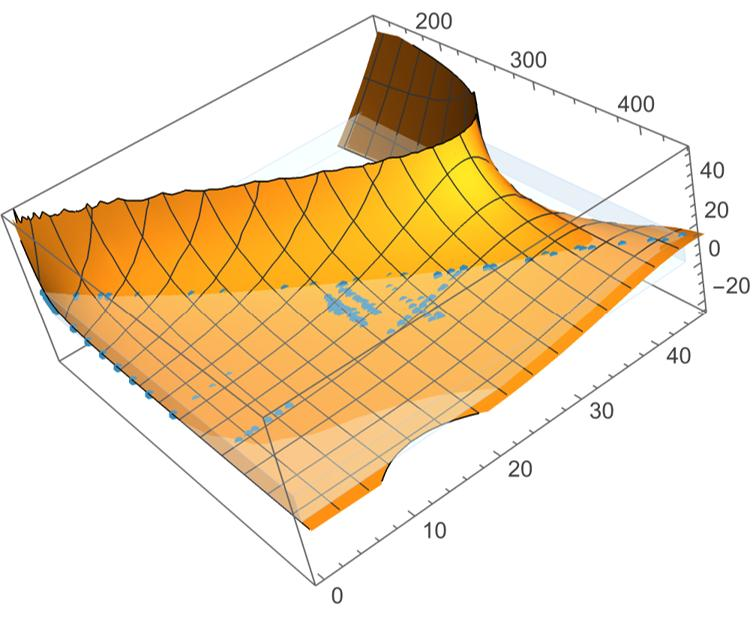
\includegraphics[width=0.9\textwidth]{SurfaceNonPhysicalPlot.jpg}
	
	\caption{Visualization of the non\textendash physical behavior inherent to the polynomial VTF surface expansion. At sufficiently high pressures the fitted surface fails to asymptotically approach zero mobility with decreasing temperature, instead exhibiting an nonphysical downturn in the predicted $\alpha$-relaxation time. This illustrates the limitations of the polynomial form used in \eqn\ref{eqn:VTFsurface}.}
	\label{figure:SurfaceNonPhysical}
\end{figure}


Even were this not the case, and it may not be for all liquids, the underlying issue remains\textemdash a polynomial expansion for the zero-mobility temperature and fragility functions, $T_{0}(P)$ and $D(P)$, is inherently non-physical. A model that better constrains the surface behavior, in particular its tendency to asymptotically approach a regime in which relaxation modes are suppressed (both for decreasing temperatures and increasing pressures), would be preferable to this simple polynomial expansion. For this reason, attention was turned toward creating a pressure–temperature dependent model of the $\alpha$-relaxation for which, regardless of the best-fit parameters, the physical requirement of an asymptotic approach to regions of zero mobility is maintained along any isobar or isotherm. For anyone familiar with developments in the glassy-dynamics community over the last few decades, the ``modified'' VTF (\eqn \ref{eqn:ModifiedVTFPressureClassic}) first suggested by Paluch \etal should come to mind\textemdash a natural analogue of the classic VTF but expressed as a function of pressure rather than temperature\cite{Paluch_1998}.
 

\begin{equation}
	\ln \langle \tau(P) \rangle
	= \ln \tau_{\infty}
	+ \frac{D_{P}\,P_{0}}{P_{0} - P},
	\label{eqn:ModifiedVTFPressureClassic}
\end{equation}

Historically, the modified VTF was introduced as a direct analogue of the classic VTF relation but reformulated for the pressure path. Paluch and co-workers demonstrated that, along an isotherm, the dramatic slowing down of molecular mobility with increasing pressure follows a divergence form that mirrors the temperature-driven Vogel--Tammann--Fulcher behavior. In this formulation, $P_{0}$ plays the role of a zero-mobility pressure, and $D_{P}$ quantifies the steepness of the divergence, thereby providing a pressure-based analogue of fragility. Because the modified VTF guarantees an asymptotic divergence of the relaxation time as $P \rightarrow P_{0}$, it naturally enforces physically reasonable behavior along every isotherm, in sharp contrast to the polynomial expansions used in \eqn\ref{eqn:VTFsurface}. This makes it particularly attractive for systems in which pressure-induced vitrification or dynamic arrest is expected, or for cases where extrapolation beyond the directly measured pressure range is required.

\subsection{Andersson--Andersson-constrained zero-mobility surface}

In \eqn \ref{eqn:VTFsurface} we introduced a Vogel--Tammann--Fulcher
(VTF) surface whose temperature--pressure curvature was constrained by
the Andersson--Andersson isochrone model fit to our \tgp data from \app \ref{app:CumeneIGP} near the glass-transition at approximately $\tau\approx 130\si{\second}$.
There, the AA model was used to enforce the physically required shape
of the boundary $T_{g}(P)$, while the VTF divergence retained its
usual temperature dependence.

Here we apply the same Andersson--Andersson model, but with a different
interpretation. Instead of modeling the glass-transition isochrone, we
assume that the \emph{zero-mobility} isochrone, the locus along which
the relaxation time diverges, shares the same AA-type curvature as
$T_{g}(P)$. The rationale is that both the glass transition and the
zero-mobility boundary reflect the same limiting physics of suppressed
structural relaxation at low temperature and high pressure.

\subsubsection*{Andersson--Andersson form for the zero-mobility isochrone}

The original AA expression for the glass-transition isochrone is as follows:
\begin{equation}
	T_{g}(P)
	= k_{1}\,\left(1 + \frac{k_{2}}{k_{3}}\,P\right)^{1/k_{2}}
	\label{eqn:AA_original}
\end{equation}
To repurpose this shape for the zero-mobility surface, we replace
$k_{1}$ by the zero-mobility temperature, or the temperature for which $\tau$ diverges to infinity, for the VTF model at 1-bar\textemdash $t_0$ from \eqn \ref{eqn:VTFsurface}.
\begin{equation}
	T_{0}(P)
	= T_{\infty}
	\left(1 + \frac{k_{2}}{k_{3}}\,P\right)^{1/k_{2}}
	\label{eqn:T0_of_P}
\end{equation}
Here $T_{\infty}=115.2\si{\kelvin}$ .  This  ensures that the zero mobility temperature provided by our AA constraint is in agreement with the 1-bar constraint from \fig  \ref{fig:cumene_VTF_1bar} as with our previous model.

The zero-mobility isochrone can equally well be expressed in terms of
the pressure required to reach divergence at a fixed temperature.  
To obtain this form, we simply solve the Andersson--Andersson expression
for $P$ rather than for $T$. 

\begin{equation}
	P_{0}(T)
	= \frac{k_{3}}{k_{2}}
	\left[\left(\frac{T}{T_{\infty}}\right)^{k_{2}} - 1\right]
	\label{eqn:P0_of_T}
\end{equation}


\subsubsection*{The AA-constrained two-variable VTF surface}

Constraining the zero-mobility isochrone introduces only two fit
parameters when used in conjunction with the 1-bar VTF constraint. It
is suggested here that a sufficient model for the relaxation dynamics of
a simple van-der-Waals liquid such as cumene, taking the form of
\eqn \ref{eqn:H_general}, requires only one additional degree of freedom\textemdash a
constant $D_{p}$ analogous to the fragility parameter $D_{0}$ in the
classical VTF expression.

\begin{equation}
	H(T,P) = \log(\tau_{\inf})
	+ \frac{D_{0}\,T_{0}(P)}{T - T_{0}(P)}
	+ \frac{D_p\,P}{P_{0}(T) - P}
	\label{eqn:H_general}
\end{equation}
Substituting \eqn \ref{eqn:T0_of_P} and \nolinebreak \eqn \ref{eqn:P0_of_T} into
\eqn\ref{eqn:H_general} gives the explicit form of \eqn \ref{eqn:H_final},
\begin{equation}
	H(T,P)
	= \log(\tau_{\inf})
	+ \frac{D_{0}\,T_{\infty}\left(1 + \frac{k_{2}}{k_{3}}\,P\right)^{1/k_{2}}}
	{T - T_{\infty}\left(1 + \frac{k_{2}}{k_{3}}\,P\right)^{1/k_{2}}}
	+ \frac{D_p\,P}
	{\displaystyle
		\frac{k_{3}}{k_{2}}
		\left[\left(\frac{T}{T_{\infty}}\right)^{k_{2}} - 1\right]
		- P },
	\label{eqn:H_final}
\end{equation}

\noindent
where $\tau_{\infty}=1.118179~\si{\pico\second}$, 
$T_{\infty}=115.201~\si{\kelvin}$, and $D_{0}=1.59655$ are fixed from the 1-bar constraint, leaving only $D_{p}$, $k_{2}$, and $k_{3}$ as degrees of freedom in the nonlinear surface fit.

The resulting parameter values are listed in \tbl  \ref{tab:Hgeneral_AA_surface_fits}.  
The corresponding fitted surface is shown in \fig \ref{fig:SurfaceZeroMobilityFit}, 
where the rear vertical isochrone surface represents the zero-mobility asymptote, 
and a second vertical isochrone surface marks the $130\,\si{\second}$ \tgp condition.  
The increasing separation between these two vertical isochrone surfaces with rising 
pressure reflects the expected decrease in fragility at higher pressures.

It is important to note that this model constitutes a zero-mobility–constrained 
surface. Both the \tgp and zero-mobility isochrones are generated using the same 
Andersson--Andersson regression; however, it is the additional modified-VTF-shaped 
constraint imposed along the isotherms that forces the relaxation dynamics to 
asymptotically approach a physically meaningful region of zero mobility for 
\emph{all} temperatures and pressures. 
This stands in sharp contrast to the earlier polynomial-expansion model, whose form 
allowed nonphysical behavior away from the data domain and did not enforce divergence 
along any thermodynamic path. 
By embedding the correct asymptotic structure directly into the surface, rather than 
attempting to approximate it with independent polynomial terms, the present model 
permits reliable extrapolation beyond the measured $(T,P)$ range. 
Such extrapolation is essential for assessing the pressure and temperature-dependent 
fragility, particularly in regions where direct measurements are not experimentally 
accessible.

\begin{figure}[!htbp]
	\centering
	\begin{tikzpicture}
		\node[anchor=south] at (0,0)
		{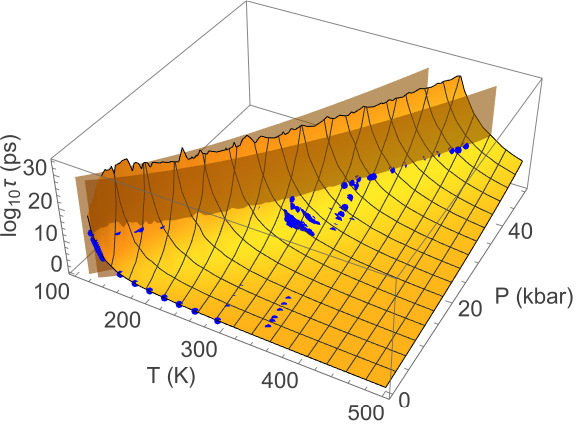
\includegraphics[width=0.92\linewidth]{Chapters/PCS/Figures/SurfaceZeroMobilityFit.png}};
		
		\node[anchor=south, yshift=2pt] at (0,12)
		{\large\bfseries Zero-Mobility Constrained Relaxation Surface};
	\end{tikzpicture}
	
	\caption[Relaxation-time surface constrained by the zero-mobility isochrone]{Fit surface resulting from the three-degree-of-freedom model of \eqn \ref{eqn:H_general}, constrained by the Andersson--Andersson representation of the zero-mobility isochrone. The rear vertical sheet represents this zero-mobility asymptote $T = T_{0}(P)$ (equivalently, $P = P_{0}(T)$), while the front vertical sheet follows the Andersson--Andersson fit to the TGP data provided in \app~\ref{app:CumeneIGP}. The curved surface shows the fitted relaxation landscape over $(T,P)$ space, with experimental data overlaid as blue points. The corresponding dataset, including percent errors defined as the deviation in $\log_{10}(\tau)$ from the fitted surface, is provided in \app~\ref{app:DPCSdata}.}
	\label{fig:SurfaceZeroMobilityFit}

\end{figure}


\begin{table}[!htbp]
	\centering
	
	\tabletitle{Fit parameters for the AA-constrained VTF surface model}
	\label{tab:Hgeneral_AA_surface_fits}
	
	\begin{tabular}{lccc}
		\toprule
		\textbf{Parameter} & \textbf{Estimate} & \textbf{Standard Error} & \textbf{t-Statistic / P-Value} \\
		\midrule
		$D_{p}$ 
		& 3.91293 
		& 0.228946 
		& $17.0911 \;/\; 3.60118\times 10^{-34}$ \\
		$k_{2}$ 
		& 1.71628 
		& 0.0125992 
		& $136.222 \;/\; 3.76332\times 10^{-135}$ \\
		$k_{3}$ 
		& 13.7721 
		& 0.213287 
		& $64.5708 \;/\; 3.49584\times 10^{-96}$ \\
		\bottomrule
	\end{tabular}
	
	\tabledescription{Fit parameters for the three-degree-of-freedom relaxation-surface model of \eqn\ref{eqn:H_general}. The table lists the parameter estimates together with their standard errors, $t$-statistics, and associated $p$-values derived from the nonlinear regression. These parameters define the Andersson--Andersson–constrained VTF surface for the zero-mobility isochrone.}
\end{table}

\begin{figure}[!htbp]
	\centering
	\begin{tikzpicture}
		\begin{axis}[
			width=0.85\linewidth,
			height=0.60\linewidth,
			xmin=0, xmax=4.7,
			ymin=120, ymax=460,
			xlabel={$P$ (\si{\giga\pascal})},
			ylabel={$T$ (\si{\kelvin})},
			grid=both,
			legend pos=north west,
			legend cell align=left,
			ticklabel style={/pgf/number format/fixed},
			]
			
			% Tg(P) data: col 2 = P (kbar), col 3 = T (K)
			\addplot[
			only marks,
			mark=*,
			mark size=2.2pt,
			mark options={blue}
			] table[
			col sep=space,
			x expr=\thisrowno{1}/10, % kbar -> GPa
			y index=2
			] {Chapters/PCS/Figures/TGPIsocroneData.txt};
			
			% Andersson--Andersson fit to Tg(P)
			\addplot[
			thick,
			dashed,
			domain=0:4.7,
			samples=200
			] {131.145*(1 + (1.64181/12.1852)*x*10)^(1/1.64181)};
			
			% Zero-mobility AA isochrone
			\addplot[
			very thick,
			red,
			domain=0:4.7,
			samples=200
			] {115.201*(1 + (1.68164/14.2038)*x*10)^(1/1.68164)};
			
			\legend{
				$T_{\mathrm{g}}(P)$ data,
				AA fit to $T_{\mathrm{g}}(P)$,
				zero-mobility AA isochrone
			}
			
		\end{axis}
	\end{tikzpicture}
	\caption[Cumene $T_{\mathrm{g}}(P)$ and AA isochrones]{
		Cumene glass-transition temperatures $T_{\mathrm{g}}(P)$ with the Andersson--Andersson fit from \app\ref{app:CumeneIGP}, together with the AA zero-mobility isochrone for comparison  (red line) shown as the rear vertical sheet in \fig \ref{fig:SurfaceZeroMobilityFit}.  The decrease in the classical isobaric fragility with increasing pressure is evident in the growing separation between these two isochronal curves.
		
	}
	\label{fig:CumeneIGP_AA_ZeroMobility}
\end{figure}

It is evident from inspection of the relaxation surface in \fig  \ref{fig:SurfaceZeroMobilityFit} that the fragility of cumene decreases with increasing pressure.  In the present framework, fragility is
defined not through the classical VTF parameters of the earlier polynomial model, but directly from
the geometry of the logarithmic relaxation surface
\begin{equation}
	H(T,P)\equiv \log_{10}\tau_{\alpha}(T,P),
\end{equation}
given by the Andersson–Andersson–constrained VTF form of \eqn \ref{eqn:VTFsurface}.
This formulation naturally allows fragility to be expressed in terms of the gradient of the surface,
thereby providing a more physical interpretation of how relaxation modes are suppressed along
isobars and isotherms.

\subsubsection*{Temperature–based scaled  fragility}
Following the scaled definition of fragility introduced in \sect\ref{sec:Fragility} (\eqn\ref{eqn:scaledfragility}), the isobaric scaled fragility is obtained by differentiating $H(T,P)$ with respect to the reduced temperature $T_{g}(P)/T$ at fixed pressure:
\begin{equation}
	m^{*}(P)
	\equiv
	\left.
	\frac{1}{\Delta}
	\frac{\partial H}{\partial\!\left( T_{g}(P)/T \right)}
	\right|_{T=T_{g}(P)}
\end{equation}
where $\Delta=\log_{10}(\tau_{g}/\tau_{\infty})$ is the scaled dynamic range between the
infinite–temperature and glass–transition relaxation times.  Because $T_{g}(P)$ is constant along an
isobar,
\[
\frac{\partial}{\partial (T_{g}/T)} = -\frac{T^{2}}{T_{g}}\,\frac{\partial}{\partial T}
\]
and therefore the scaled  fragility can be written compactly in terms of the gradient of the relaxation
surface:
\begin{equation}
	\label{eqn:mpstar_surface}
	m^{*}(P)
	=
	-\frac{T_{g}(P)}{\Delta}
	\left.
	\left( \nabla H \right)_T
	\right|_{T=T_{g}(P)}
\end{equation}

Physically, this quantity reflects how rapidly the dynamics slow when the temperature is decreased
slightly below $T_{g}(P)$ at fixed pressure.  Because small variations in temperature do not strongly
modify the underlying potential–energy landscape near the glass transition, $m^{*}(P)$ primarily
characterizes the \emph{probe response} of the system—how sharply the available relaxation pathways
become dynamically inaccessible as thermal energy is withdrawn. A strong argument was made previously for the adoption of the scaled fragility definition given in \eqn \ref{eqn:scaledfragility}. Nevertheless, to facilitate direct comparison between fragility values derived from the present surface and those reported elsewhere in the literature, it is appropriate to continue working with the classical Angell definition of fragility. Accordingly, results will primarily be discussed in terms of the conventional fragility, although, where easily accommodated, both definitions will be presented.

Before proceeding to an analysis of the pressure dependence of isobaric fragility, it is first necessary to address the fragility of cumene at atmospheric pressure. Reported values of this parameter exhibit a notable degree of variability within the literature, even after accounting for differences in how the glass transition temperature is defined, with most studies adopting the standard criterion of $\tau = 100\,\si{\second}$. Understanding the origin of this discrepancy serves not only to validate the surface model developed here, which relies critically on a fixed isobaric regression at atmospheric pressure, but also to reinforce a conclusion that is already well established in the literature. Specifically, light scattering experiments, as a non-invasive probe, provide a more faithful measure of the intrinsic $\alpha$-relaxation associated with the stochastic thermal evolution of the system, even in a comparatively simple liquid such as cumene, which might otherwise be expected to lend itself equally well to dielectric spectroscopy and DPCS.

Our surface model, anchored by a 1--bar VTF regression, relies on data collected by Hansen \etal \cite{Hansen2018} and Li \etal \cite{Li1995CumenePRL}, together with the \tgp point derived from the Andersson--Andersson fit described in \app\ref{app:CumeneIGP}. \fig  \ref{fig:cumene_VTF_1bar} demonstrates remarkably good agreement between the model and the data over the full dynamic range. A slight tendency for the VTF fit to underestimate the data is observed as temperatures approach $160\,^{\circ}\mathrm{C}$; however, this region lies near the upper operational limit of Brillouin light scattering, where the extracted relaxation times begin to approach the Bose peak. Consequently, confidence in these intermediate--temperature points is reduced.

Importantly, a substantial body of ambient--pressure data exists for cumene, and the 1--bar datasets employed here were selected specifically because they were obtained using light--scattering probes\textemdash DPCS in the case of Hansen \etal and Brillouin light scattering in the work of Li \etal The \tgp point would likewise be expected to provide a direct measure of the structural relaxation, as few experimental observations are more direct than the physical vitrification of the material. However, as discussed previously in the description of the surface model, the precise relaxation time $\tau_i$ associated with this isochrone is not directly experimentally measurable and is instead constrained by where it crosses this atmospheric VTF isobar. The corresponding isochronal value is nonetheless independently verifiable in the case of cumene via the intercept obtained from the thermodynamic scaling of the data shown in \fig \ref{figure:tdscaling}.

\iffalse
The strong adherence of our data to a VTF description, shown in \fig \ref{fig:cumene_VTF_1bar}, may be contrasted with the behavior inferred from dielectric spectroscopy in the work of Chen and Richert~\cite{Chen}. That study had a different focus and did not report new measurements of the relaxation dynamics of cumene (iso-propylbenzene), but instead compiled bulk dielectric and viscosity data from three prior sources. These compiled data were used to extract a classical Angell fragility for cumene of $m=77.6$, a comparatively high value relative to others reported in the literature.

It is important to emphasize, however, that this fragility does not arise from the slope of a single global VTF fit applied over the full temperature range of the compiled dataset. As shown in \fig \ref{fig:Chen_global_VTF}, a global VTF regression significantly overestimates the relaxation times in the intermediate-temperature regime while underestimating the data in the region of faster dynamics. This stands in marked contrast to the fidelity demonstrated by the VTF fit to the Hansen \etal and Li \etal light-scattering data in \fig \ref{fig:cumene_VTF_1bar}. Such behavior is not unexpected: the low-viscosity regime lies within the optimal sensitivity range for Brillouin light-scattering measurements, while simultaneously approaching the practical limits of dielectric spectroscopy due to both instrumental bandwidth constraints and possible overlap with secondary fast relaxation processes.

Although a fragility may be formally extracted from the global VTF fit, yielding a notably high value of $m=91$, fragility is fundamentally defined by the slope of the relaxation dynamics at the glass transition, rendering curvature far from this transition of limited relevance. Accordingly, Chen and Richert adopted the more robust approach of fitting the VTF equation exclusively to data within the viscous regime approaching $T_g$. This restricted fitting window, together with the corresponding ``viscous'' VTF regression, is indicated by the shaded region in \fig \ref{fig:Chen_global_VTF}. When fragility is determined solely from data within this regime, a more moderate value of $m=74$ is obtained, in closer alignment with physical expectations.

\definecolor{cumeneMagenta}{RGB}{170,60,170}
\begin{figure}
	\centering
	\begin{tikzpicture}
		\begin{axis}[
			width=0.80\linewidth,
			height=0.60\linewidth,
			xmin=120,
			xmax=350,
			ymin=0,
			ymax=16,
			xlabel={$T$ (K)},
			ylabel={$\log_{10}\tau_{\alpha}$ (s)},
			legend pos=north east,
			legend cell align=left,
			grid=both,
			ticklabel style={/pgf/number format/fixed},
			]
			
			%------------------------------------------------------------
			% Data set 1: open purple triangles
			%------------------------------------------------------------
			\addplot[
			only marks,
			mark=triangle,
			color=purple,
			mark options={draw=cumeneMagenta, fill=none},
			]
			table[
			x=triangleX,
			y=triangleY,
			col sep=comma,
			]{ChenVTF.csv};
			\addlegendentry{Barlow \cite{Barlow}}
			
			%------------------------------------------------------------
			% Data set 2: open purple circles
			%------------------------------------------------------------
			\addplot[
			only marks,
			color=purple,
			mark options={draw=cumeneMagenta, fill=none},
			]
			table[
			x=openX,
			y=openY,
			col sep=comma,
			]{ChenVTF.csv};
			\addlegendentry{Gangasharan \cite{Gangasharan}}
			
			%------------------------------------------------------------
			% Data set 3: closed purple circles
			%------------------------------------------------------------
			\addplot[
			only marks,
			mark=*,
			color=purple,
			mark options={draw=cumeneMagenta, fill=purple},
			]
			table[
			x=closedX,
			y=closedY,
			col sep=comma,
			]{ChenVTF.csv};
			\addlegendentry{Nielsen \cite{Nielsen}}
			
			%------------------------------------------------------------
			% Global VTF regression fit (your fitted parameters):
			% y = a + B/(T - c)
			% B = 305.881, a = -.724953, c = 107.395
			%------------------------------------------------------------
			\addplot[
			red,
			thick,
			domain=120:350,
			samples=200,
			]
			{ -.724953 + 305.881/(x - 107.395) };
			\addlegendentry{VTF (global)}
			
			%------------------------------------------------------------
			% Vicous VTF regression fit (your fitted parameters):
			% y = a + B/(T - c)
			% B = 600.143, a = -4.62659, c = 95.5547
			%------------------------------------------------------------
			\addplot[
			blue,
			thick,
			dashed,
			domain=120:350,
			samples=200,
			]
			{ -4.62659 + 600.143/(x - 95.5547) };
			\addlegendentry{VTF (viscous)}
			
			%------------------------------------------------------------
			% Equation box (kept identical to your style)
			%------------------------------------------------------------
			\node[
			anchor=north east,
			fill=white,
			draw=black,
			rounded corners=2pt,
			inner sep=4pt
			]
			at (rel axis cs:.98,0.65)
			{%
				$\displaystyle
				\ln\tau = \ln\tau_{\infty}
				+ \frac{D T_{0}}{T - T_{0}}$
			};
			
			%------------------------------------------------------------
			% Shaded region indicating viscous-fit temperature window
			%------------------------------------------------------------
			\addplot [
			draw=none,
			fill=gray,
			fill opacity=0.15,
			]
			coordinates {
				(120,0)
				(155,0)
				(155,16)
				(120,16)
				(120,0)
			};
			
			
		\end{axis}
	\end{tikzpicture}
	
	\caption{Atmospheric-pressure relaxation data for cumene compiled by Chen and Richert, plotted as $\log_{10}\tau_{\alpha}$ versus temperature\cite{Chen}. With the exception of the data of Barlow \cite{Barlow}, which consist of viscosity measurements converted to relaxation times via the Maxwell relation using a constant high-frequency shear modulus $G_{\infty}=0.04\,\text{GPa}$, all data shown were obtained via dielectric spectroscopy. The solid red curve represents a single VTF regression applied over the full temperature range of the compiled dataset.  However, this global fit does not adequately capture the behavior of the data in the low-viscosity (high-temperature) regime. The fragility value of $m=77.6$ reported by Chen and Richert was therefore obtained from a VTF fit restricted to the viscous regime near the glass transition, indicated by the shaded region, with the corresponding VTF regression shown by the dashed blue curve.}
	
	\label{fig:Chen_global_VTF}
\end{figure}

The slightly higher value of $m=77.6$ reported by Chen and Richert reflects their particular selection of data within this viscous regime. While the specific rationale for excluding a substantial fraction of the available viscous-domain data is not explicitly discussed, such a choice may reasonably be motivated by an effort to avoid disproportionate weighting of data clustered near the glass transition or to maintain a more uniform spacing of points in the fitting procedure. Regardless of the motivation, this selective treatment introduces a nontrivial variation in the extracted fragility, underscoring the sensitivity of fragility to both the chosen fitting window and the details of the fitting methodology.

The purpose of the preceding discussion has been to clarify the rationale behind our choice to anchor the atmospheric-pressure VTF isobar of the surface model using light-scattering data, despite the more limited availability of such measurements within the literature, as well as to make the argument for why light scattering is, even in the case of cumene, and arguably superior probe of structural relaxation dynamics. While it is well established that differing values of fragility may be obtained depending on the experimental probe, or even minor differences in data analysis, fragility itself is not a sharply defined material constant in the same sense as, for example, the speed of sound or the location of a first-order phase transition. Rather, it is derived from the behavior of a second-order glass transition and is therefore inherently more sensitive to both experimental methodology and data treatment. Nevertheless, fragility remains a quantity of significant physical interest, and if  confidence is to be placed in values extracted from a surface construction, it is essential that the limiting cases such as the atmospheric-pressure constraint be as reliable as possible.

Cumene, by virtue of its molecular simplicity and predominantly van der Waals interactions, might reasonably be expected to be equally amenable to characterization by dielectric spectroscopy and light-scattering techniques. There is, however, no fundamental guarantee that a phenomenological form such as the VTF equation should accurately describe structural-relaxation data spanning fourteen decades in time. Even so, the light-scattering measurements of Hansen \etal and Li \etal are more uniformly and robustly described by VTF regression over their experimentally accessible dynamic range than are corresponding dielectric-based compilations. Given both the indirect nature of dielectric spectroscopy and its practical limitations as the dynamics approach the high-frequency regime, it is therefore reasonable to construct the atmospheric-pressure constraint of the surface model using light-scattering data. Doing so increases confidence not only in the extracted atmospheric fragility but also in the associated $\alpha$-relaxation times and derived quantities that depend on this limiting behavior. More generally, dielectric spectroscopy and depolarized photon-correlation spectroscopy probe distinct relaxation channels, and parameters such as fragility are intrinsically sensitive to how these channels are weighted. Consequently, while dielectric spectroscopy remains an essential and broadly applicable technique, light-scattering methods, where experimentally accessible, provide a more direct and reliable measure of collective glassy dynamics.


\fi
\subsubsection*{Pressure dependence of fragility}
The surface model defined in \eqn \ref{eqn:H_final} provides a robust and internally consistent framework for examining the pressure dependence of isobaric fragility. In the discussion that follows, we focus primarily on the conventional Angell fragility in order to facilitate direct comparison with previously reported literature values. For completeness, the pressure dependence of both the conventional fragility and the scaled fragility $m^{*}(P)$ defined in \eqn \ref{eqn:mpstar_surface} are shown in \fig  \ref{figure:fragilityPressure}. 

At ambient pressure, the fragility extracted from the present surface lies slightly below commonly cited values for cumene. Dielectric analyses typically report fragilities in the range $m \approx 70$--$80$, for example $m = 77.6$ as obtained by Chen and Richert \cite{Chen}, and values near $m \approx 70$--$75$ as compiled by Wang \etal \cite{Wang}. In contrast, light-scattering-based determinations, such as those derived from Brillouin and photon-correlation measurements of cumene \cite{Li1995CumenePRL}, tend to yield somewhat lower values. This difference is likely also partially attributable to the manner in which fragility is evaluated within the present framework. Specifically, the fragility reported here is obtained directly from the local gradient of the relaxation-time surface, rather than from fits restricted exclusively to the viscous regime. As a consequence, the resulting value is sensitive to the overall goodness of fit across the accessible dynamic range, rather than being dominated by enforced low-temperature curvature alone.

\begin{figure}[!htbp]
	\centering
	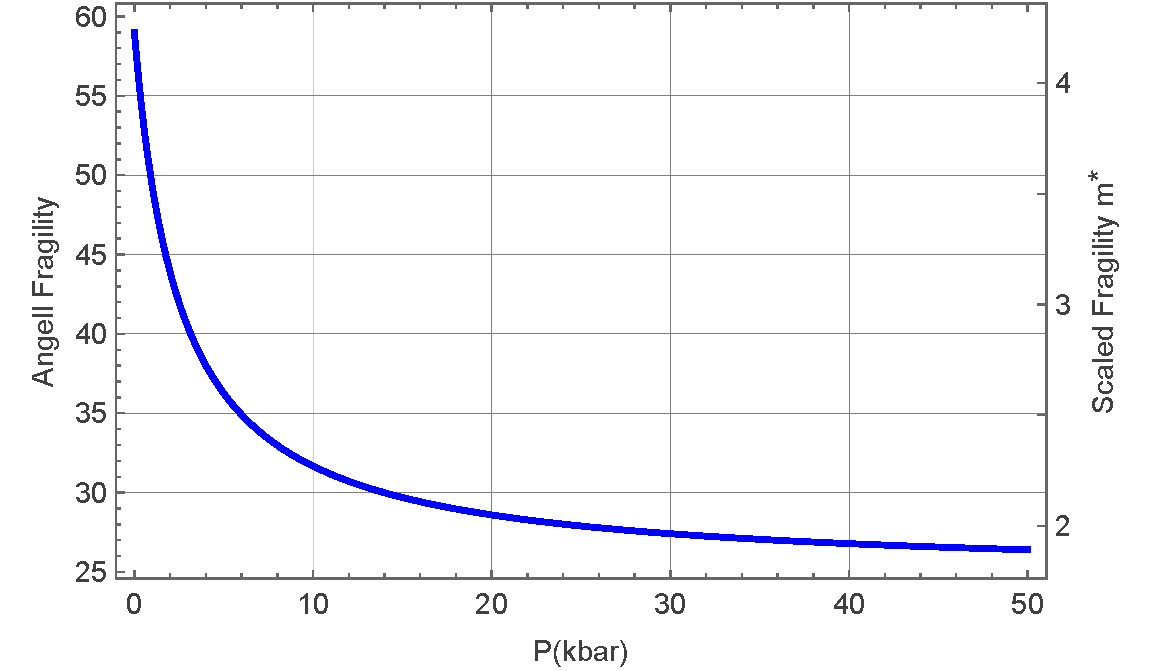
\includegraphics[width=0.9\linewidth]{PressureVsFragility.pdf}
	\caption{
		Pressure dependence of the isobaric fragility of cumene obtained from the relaxation-time surface. The left axis shows the conventional Angell fragility $m$, while the right axis displays the scaled fragility $m^{*}$ defined in \eqn \ref{eqn:mpstar_surface}. When viewed in terms of the scaled fragility, the data clearly suggest an asymptotic approach toward a finite high-pressure limit that retains more fragility than would arise from purely Arrhenius behavior.
	}
	\label{figure:fragilityPressure}
\end{figure}


Despite this modest reduction in magnitude at low pressure, the qualitative pressure evolution of the fragility is clear and robust. The fragility exhibits a smooth but distinctly nonlinear decline with increasing pressure, consistent with the growing separation between the glass-transition isochrone $T_g(P)$ and the zero-mobility isochrones shown in \fig  \ref{figure:SurfaceFit}. With increasing pressure, the system becomes progressively stronger, approaching Arrhenius-like behavior, consistent with a stiffening of the underlying relaxation landscape.

One particularly striking feature of this model is the emergence of a high-pressure asymptote as demonstrated in \sect \ref{sec:asymptote}. It is often implicitly assumed that increasing pressure yields a stronger liquid, with the limiting case being purely Arrhenius behavior. Although the fragility of cumene decreases rapidly as cooperative dynamics are suppressed, these dynamics do not appear to be fully eliminated. The limiting fragility obtained from the surface model of \eqn \ref{eqn:H_final} as pressure approaches infinity is approximately $m^* = 1.8$, corresponding to $m = 25$ in terms of the conventional Angell fragility. This represents a clear instance in which the utility of the scaled fragility defined in \eqn \ref{eqn:scaledfragility} becomes evident. As shown in \fig  \ref{figure:fragilityPressure}, even without extrapolation beyond the experimentally accessible data, the scaled fragility is clearly converging toward a value significantly greater than unity. This limiting behavior remains distinctly more fragile than that of a purely Arrhenius system, indicating that increasing pressure does not drive the liquid into a truly strong glass-forming regime. Instead, the surface model suggests the persistence of residual non-Arrhenius character even at very elevated pressures, consistent with an energy landscape that becomes increasingly stiff while retaining a finite degree of dynamical heterogeneity.

The existence of this asymptotic fragility is not imposed by the model but rather it emerges naturally from the global structure of the relaxation-time surface. The rapid approach toward this asymptote well within the domain of the available relaxation data lends confidence to its physical significance. At least in the case of cumene, it appears that the system cannot be driven fully into Arrhenicity by the application of pressure alone.


\subsubsection*{Isothermal pressure–modified fragility}

An entirely analogous expression follows for compression along isotherms. Defining the glass--transition pressure $P_{g}(T)$ via $H\!\left(T,P_{g}(T)\right)=\log_{10}\tau_{g}$, the pressure--modified fragility is defined with respect to the reduced pressure and may be written as
\begin{equation}
	m^{*}_{P}(T)
	\equiv
	\left.
	\frac{1}{\Delta}
	\frac{\partial H}{\partial (P/P_{g}(T))}
	\right|_{P=P_{g}(T)}
	=
	\frac{P_{g}(T)}{\Delta}
	\left.
	(\nabla H)_P
	\right|_{P=P_{g}(T)}
\end{equation}


In contrast to temperature variation, increasing pressure directly alters the intermolecular structure: local cages tighten, barrier heights increase, and the potential–energy landscape itself is reshaped. Thus $m^{*}_{P}(T)$ represents a \emph{susceptibility of the landscape to mechanical compression}, rather than a probe of dynamical accessibility.

For this reason, it is the opinion of the author that the isothermal pressure--modified fragility should be understood as fundamentally \emph{not} a measure of landscape fragility; rather, it quantifies how readily the landscape itself deforms under pressure—no more a ``fragility'' than EMF is a force. Even so, it remains a useful parameter when investigating vitrification under compression, particularly as one approaches pressures for which all relaxation modes are suppressed and the structural entropy becomes effectively locked in. This ``pressure quenching'' is, in many cases, a more practical route to rapid vitrification when thermal quenching is too slow to avoid crystallization.

\subsubsection*{Connection to activation volume}

The same isothermal pressure derivative that defines the pressure--modified fragility also
appears naturally in the conventional definition of the activation volume.
For a relaxation process described by
$\tau(T,P)$, the molar activation volume is defined as
\begin{equation}
	\label{eqn:activationVolume}
	\Delta V^{\ddagger}(T,P)
	\equiv
	RT
	\left.
	\frac{\partial \ln \tau(T,P)}{\partial P}
	\right|_{T},
\end{equation}
where $R$ is the universal gas constant.
Expressed in terms of the surface 
$H=\log_{10}\tau$ implemented here, \eqn\ref{eqn:activationVolume} becomes

\begin{equation}
	\Delta V^{\ddagger}(T,P)
	=
	(\ln 10)\,RT
	\left.
	(\nabla H)_P
	\right|_{T}.
\end{equation}

Evaluated along the glass--transition isochrone $P=P_{g}(T)$, the activation volume is therefore
directly proportional to the same local surface derivative that enters the definition of the
pressure--modified fragility:
\begin{equation}
	\Delta V^{\ddagger}_{g}\!\left(T,P_{g}(T)\right)
	=
	(\ln 10)\,R\,T\,
	\frac{\Delta}{P_{g}(T)}\,
	m^{*}_{P}(T).
	\label{eqn:mpstar_activationVolume}
\end{equation}

This relation makes explicit that $m^{*}_{P}(T)$ provides a scaled measure of the pressure sensitivity of the dynamics, normalized by the glass--transition pressure and the accessible dynamic range. When combined with the appropriate thermodynamic prefactors, it yields the conventional activation volume $\Delta V^{\ddagger}_{g}(T,P)$, which retains its usual interpretation as a molar volume characterizing pressure--induced slowing of the structural dynamics.

Within the surface--based framework developed here, activation volume and modified fragility are
thus revealed to be complementary projections of the same relaxation--surface gradient.
The distinction lies not in the derivative itself, but in the physical interpretation imposed by the
choice of scaling: multiplication by $P_{g}(T)$ yields a scaled susceptibility describing how
readily the relaxation landscape deforms under compression, whereas multiplication by $RT$
recovers the conventional activation volume familiar from high--pressure relaxation studies.
This unification clarifies the relationship between pressure fragility and activation volume without
requiring separate fits or auxiliary models, and highlights the utility of the constrained surface in
providing physically consistent derivatives across the full $(T,P)$ domain.

\subsubsection*{Isochronic fragility and surface geometry}

The preceding measures of fragility emphasize either thermal variation at fixed pressure or mechanical compression at fixed temperature. A more neutral characterization follows by considering variations taken \emph{along an isochrone} of the relaxation surface itself. Within the present framework, this quantity arises naturally from the local geometry of the surface $H(T,P)$ and requires no additional fitting assumptions.

Along an isochrone defined by $H(T,P)=\log_{10}\tau=\mathrm{const}$, the total differential vanishes,
\begin{equation}
	\left.
	\frac{\partial H}{\partial T}
	\right|_{P} dT
	+
	\left.
	\frac{\partial H}{\partial P}
	\right|_{T} dP
	=0,
\end{equation}
so that the slope of the isochrone in the $(T,P)$ plane is given by
\begin{equation}
	\label{eqn:isochronicSlope}
	\left.
	\frac{dP}{dT}
	\right|_{H}
	=
	-
	\frac{
		\left(\partial H/\partial T\right)_{P}
	}{
		\left(\partial H/\partial P\right)_{T}
	}.
\end{equation}

This ratio of surface–gradient components provides a direct measure of the relative influence of temperature and pressure on the dynamics at fixed relaxation time and may be identified as an isochronic fragility. Unlike isobaric or isothermal measures, this quantity does not privilege a particular thermodynamic path, but instead reflects the intrinsic geometry of the relaxation surface.

If an equation of state is invoked to transform the surface from $(T,P)$ to $(T,V)$ coordinates, an equivalent isochronic fragility may be obtained in terms of the slope of constant--$\tau$ contours in $(T,V)$ space. In this representation, the separation between thermal and volumetric contributions to the dynamics becomes explicit, and the conventional isochoric fragility discussed in the literature is recovered as a particular projection of the same surface geometry. The agreement between these equivalent constructions emphasizes that isochronic, isobaric, and isochoric fragilities are not independent material properties, but rather complementary manifestations of the same underlying relaxation landscape.
